\chapter{High mobility material}

\chapter{Scanning Tunneling Microscopy (STM)}
	\section{Theory of STM and Techniques}
\subsection{grid map}
\subsection{STM noise}
\section{STM System in this Study}
%note: talk about the sample plate. 
\footnote{Supplementary: Major Fix of Createc Documentation}
\section{STM as a probe for electron scattering}

\section{STM and transport: 2D and 3D}
From 2D to 3D, what can we say from STM and what we can not. 
1) defect density-> cleaving, scanning etc induced impurities. 2D surface defect number may not represent the bulk-> more 3D materials. 
2) defect scattering -> All defect scattering in STM will reflect to the bulk. 


\chapter{Introduction to PtSn\textsubscript{4}}
	\section{Crystal Structure and Preparation}
	\section{Crystalline Symmetry and Band Structure} 
%todo: write about how PtSn4 bonds, with interlayer bonding not merely van der Waals force but metallic bonds. 
\footnote{Theory Calculations and Previous ARPES Study}
	\section{PtSn\textsubscript{4} as a Material with High Electron Mobility}
	\footnote{Transport Measurements and Previous Studies}

\chapter{STM Measurements of PtSn\textsubscript{4}}
\section{Sample Preparation}

\par Sample preparation is one of the keys to a successful STM experiment. As the surface of the sample is what we are trying to probe, making sure the surface is as clean and stable as possible is usually the goal of sample preparation. 

\par We achieve a clean and stable crystal surface via in-situ cleaving, it is worth mentioning that prior to the successful room-temperature cleaving, we did 2 trials of low-temperature cleaving at around 20K and the they failed, thus we will elaborate the in-situ root-temperature cleaving we performed. We first prepare the sample on bench, a mushroom like sample holder made of oxygen free copper is used. You can see a stacking structure on the left of \ref{fig:ch4_cleaves} a), from bottom to top the components are sample holder, a Pt-sheet, PtSn$_4$ single crystal, a cylindrical MACRO ceramic post. Each components are attached to the neighbors via EPO-TEK H20E, a 100 percent solid silver-filled epoxy with low contact resistance. A polycrystalline gold is mounted next to the assembly serving as a reference metal and a tip cleaning surface. 

\par As discussed in Ch.3, despite having a layered structure, the inter-layer bonding is not merely weak van der Waals force, but rather metallic, making PtSn$_4$ not easily cleavable. To increase the success rate, a Pt-sheet is mounted as a buffer layer between the sample holder and the crystal. The copper sample holder has a rough surface with some residual of silver epoxy which is hard to remove, the Pt-sheets offers a cleaner interface for the epoxy polymer-network to form. And the downside of having another epoxy layer between copper sample holder and the sheet is compensated by the large Cu-Pt interface area. Therefore, cleaving on Pt-sheet gives a larger chance for a successful cleave and thus lays the foundation for the \ac{STM} experiments in this study. It is also worth mentioning that all silver epoxies are cured at the same optimal condition for good consistency. 

\begin{figure}
	\centering
	\includegraphics[width=0.8\textwidth]{Ch4_cleaving.pdf}
	\caption{Cleaving of PtSn$_4$, Pre-cleaving and post-cleaving of the first trail with only HR$_1$ sample a), b). Pre-cleaving and post cleaving of the second trial with dual sample side by side, left is the HR$_2$ and right the LR$_1$ sample. }
	\label{fig:ch4_cleaves}
\end{figure}

\par The sample holder is then mounted to the sample plate and transferred into the preparation chamber, which sits at a pressure near $10^{-10}$ mbar and at room-temperature (we tried low temperature cleaving at T~20K but the post fall off with the crystal surface intact, indicating that the inter-layer bonding of the crystal is stronger than the crystal-epoxy-post bonding at low temperature), then we drive one of our arms horizontally towards the downward facing sample-post assembly with directions indicated as red arrows shown in a) and c) of \ref{fig:ch4_cleaves}, the cleaving results are shown in b) and d), where we inspected the crystal in-situ with a K2 camera right after the cleave. The cleaved crystals reveals large shiny areas with some cracks in between, during the experiments, we will land our tips onto the surface of the shiny areas. 

\par In total, our data were collected in 2 experiments, the first experiment is on the slow-cooled sample(shown in a) of \ref{fig:ch4_cleaves}), the second experiment is on a dual sample plate with slow-cooled sample (the same sample but recleaved) and a fast-cooled sample in comparison (shown in c) of \ref{fig:ch4_cleaves}). So, in total, we did 3 cleaves on 2 different samples (2 on slow-cooled  (highRRR) and 1 on fast-cooled (lowRRR) samples), since each cleave correspond to a new surface to explore, from now on, we will refer them as highRRR$_1$(HR$_1$), highRRR$_2$(HR$_2$), and lowRRR$_1$(LR$_1$).


\section{Topography overview}
\par In the course of the study of PtSn$_4$, we went through a several phases, with firs phase being about the surface exploration, termination determination, scanning parameter optimization, and some spectroscopy measurements conducted on HR$_1$. The second phase was conducted on HR$_2$ and LR$_1$, with the focus on characterizing the defect scattering behaviors on both surfaces through topography and spectroscopy measurements. This section will cover the topographical aspect of this study. 

\begin{figure}
	\centering
	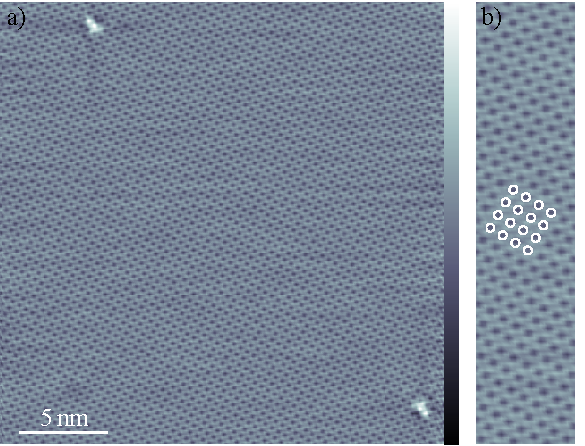
\includegraphics[width=\textwidth]{Ch4_Pristine_PtSn4.pdf}
	\caption{ }
	\label{fig:ch4_pristinetopo}
\end{figure}

\par In total, we took over 20000 STM topographies in this study, covering an area of over two million nanometer squared. More specifically, we acquired around 10000 images on 5 macroscopic spots on the HR$_1$ surface, around 5000 images on the HR$_2$ surface, and around 2000 images on 2 macroscopic spots on the LR$_1$ surface. 
Panel a) of \ref{fig:ch4_pristinetopo} exhibits a typical STM topography on PtSn$_4$, it is featured by waffle-like square corrugations and sparse defects at different atomic sites. Pristine cleaved surfaces are remarkably defect free, which we quantify through a careful statistical analysis in a subsequent section. We can overlay the Pt-layer to the surface of the pristine surface as shown in b) of \ref{fig:ch4_pristinetopo} and it maps perfectly with the square corrugations we observed. It might be tempting to say that we are typically scanning on the Pt-surface, but note that as mentioned in Ch.2, the tunneling current of STM has both the contribution of distance and electronic structure of the sample, the pattern revealed on topography is not necessarily the top most surface. To determine on what termination we are scanning, we ran a full terrace characterization.

\begin{figure}
	\centering
	\includegraphics[width=0.5\textwidth]{example-image-a} % Replace with your image file
	\caption{Placeholder for cleaving planes of PtSn$_4$}
	\label{fig:ch4_cleavingplane}
\end{figure}


\subsection{Terrace determination}
%todo: to insert the pdf showing potential cleaving planes of PtSn4.
\par Surface of PtSn$_4$ reveals flat terraces that belongs to different cleavage planes. Inspecting the crystal structure of PtSn$_4$, we note that there are three possible cleavage planes as shown in Fig 2. They are Sn$_a$-Pt, Pt-Sn$_b$, and Sn$_b$-Sn$_a$. Sn$_b$-Sn$_a$ bond has twice the length as Sn$_a$-Pt and Pt-Sn$_b$ bond and thus is weaker. We expect this material to cleave predominately between Sn$_b$-Sn$_a$. 

\begin{figure}
	\centering
	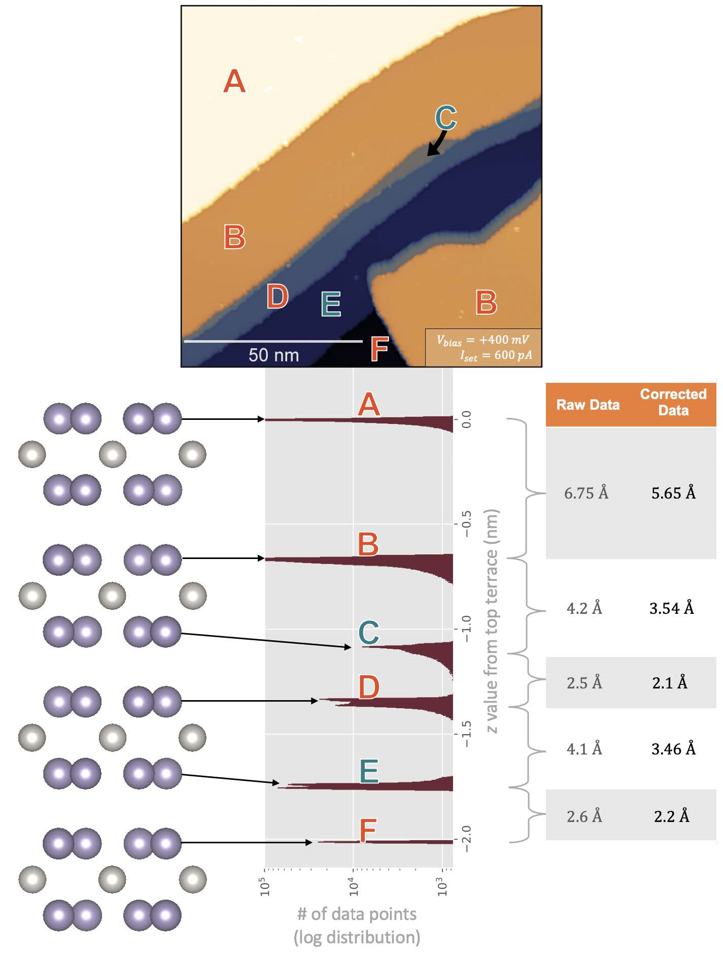
\includegraphics[width=\textwidth]{Ch4_termination.png}
	\caption{termination characterization}
	\label{fig:ch4_termination}
\end{figure}

\par In the experiment, we often landed our tips on a dominating terrace that is big and flat, and by scanning the step edges of the terraces, we could also see other terminations but with much less occurrence. To determine the dominating terrace we are scanning, we analyzed the step heights on a step-edge area, as shown in \ref{fig:ch4_termination}. 

Before we discuss the result shown in panel b) of \ref{fig:ch4_termination}, we need to understand how cleaving modifies the sample structure. Note that cleaving breaks the translational symmetry for the top layers; this effect is most profound for the surface layer where the covering layers are replaced by vacuum; the absence of support from the covering layers results in the surface layer to 'relax' into the surface, making the physical distance between the top most layer and the subsequent layer smaller than that of the normal lattice. However, how strong the relaxation effect is varies for different cleavage planes with different local bonding environments. There are two possible Sn-terminations in PtSn$_4$, and it is clear that compared to the relaxation of the Sn$_a$ termination due to Sn$_b$-Sn$_a$ cleaving, a Pt-Sn$_b$ cleaving will lead to a larger relaxation for the Sn$_b$ termination, as illustrated in \ref{fig:ch4_relaxation}. As a consequence, the relaxed height difference between Sn$_a$-Sn$_b$ terminations will be larger than 2.8 {\AA} (1/4 unit cell along the $b$-axis), and that of Sn$_b$-Sn$_a$ will be smaller than 2.8 {\AA}. That is precisely what we see in the height profile of step edge areas in panel b) of \ref{fig:ch4_termination}. Here, a height histogram is mapped from the topography and peaks can be assigned to different terminations. This analysis confirmed that the Sn$_a$ is the dominant termination we are scanning. Other terminations corresponding to the Pt and Sn$_b$ layer were seldom observed, accounting for less than 1\% of the total area investigated. 

\par For more details of the termination determination of PtSn$_4$, the reader can consult chapter 3 of Ashley Warner's thesis \cite{warner_defect_nodate}.

\begin{figure}
	\centering
	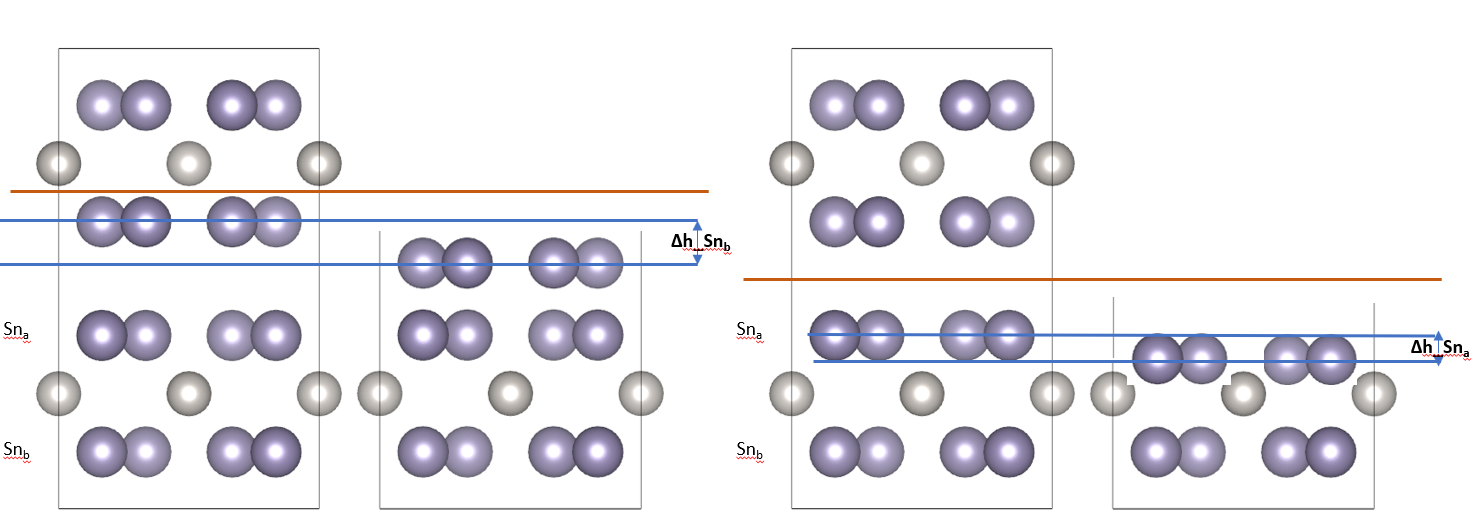
\includegraphics[width=\textwidth]{Ch4_relaxation.png}
	\caption{Relaxation}
	\label{fig:ch4_relaxation}
\end{figure}



\section{Defect Analysis}

\subsection{Defects in STM}
what is a defect?
Phenomenologically, defects are any disruptions in ideal, periodic lattice arrangement in STM topography. They can have different origins; for point defects, they can be due to site vacancy, substitution, adatoms on the surface, or interstitials that reside between layers.
Lattice imperfection breaks the local translational symmetry and is one the major sources of electron scattering in a metallic system. As the electron-phonon scattering and electron-electron scattering got supressed in low temperature, the temperature independent electron-defect scattering term dominates the residual resistance. Therefore, characterizing the defects in PtSn4 is crucial to understand the low temperature limit of resistance. In real space, electron-defect scattering process results in the outgoing electron being scattered with a modulated momentum and will thus create interference patterns around the scattering center, this modulation can be directly observed with STM spectroscopy, as the signal of differential conductance is proportional to the local density of state (LDoS) of electron. 
However, not all defects observed in STM can be considered a scattering center for the bulk material, as some defects can only reside on the surface or can be an artifact introduced by STM experiments.  For example, the adatoms defects are purely surface, with the cause being surface contamination either from the vacuum environment or from the tip, the adatom will never be observed in the bulk. 
In this study, we first identify different types of defects via topographic images, then we take point spectroscopy measurement on the defects ,and grid maps around defect rich areas to characterize their scattering behavior. In this section, we will present all the point defects types we observed in PtSn$_4$ and the their density via rigorous statistical analysis. 

\begin{figure}
	\centering
	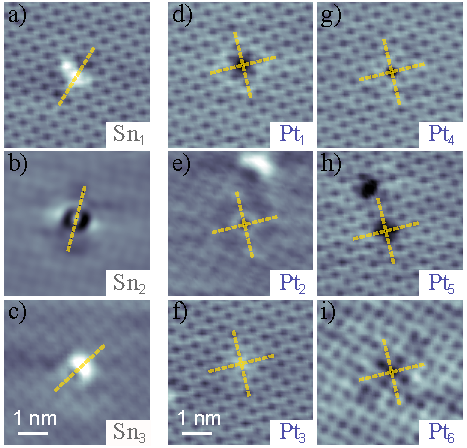
\includegraphics[width=\textwidth]{Ch4_defect_gallery.pdf}
	\caption{defect gallery}
	\label{fig:ch4_defectgallery}
\end{figure}

\subsection{Defects Topography}
Throughout the exploration on both fast-cooled and slow-cooled sample, different types of defects are observed, with the dominating source being point defects. In total, we observed 9 types of point defects in PtSn$_4$ as shown in \ref{fig:ch4_defectgallery}. 6 types are characterized as reside on Pt-sites and 3 on the Sn-site. Whether the defect belongs to a Sn-site or a Pt-site is determined with the lattice symmetry preserved in the Pt-layer and Sn-layer. As shown in \ref{fig:ch4_symmetry}, point defects sitting at the Pt-site will break the local translational symmetry, it changes the local electronic environment of 4 neighboring Pt atoms and thus exhibits a 2 fold symmetry and mirror symmetry in 2 axes(C$_2v$). As for Sn-layers, a modification on the Sn-site will result in a pattern with lower symmetry, with mirror symmetry in only 1 axis. Therefore, we can determine the origin of the defect based on the symmetry exhibited by the defect topography. 

\begin{figure}
	\centering
	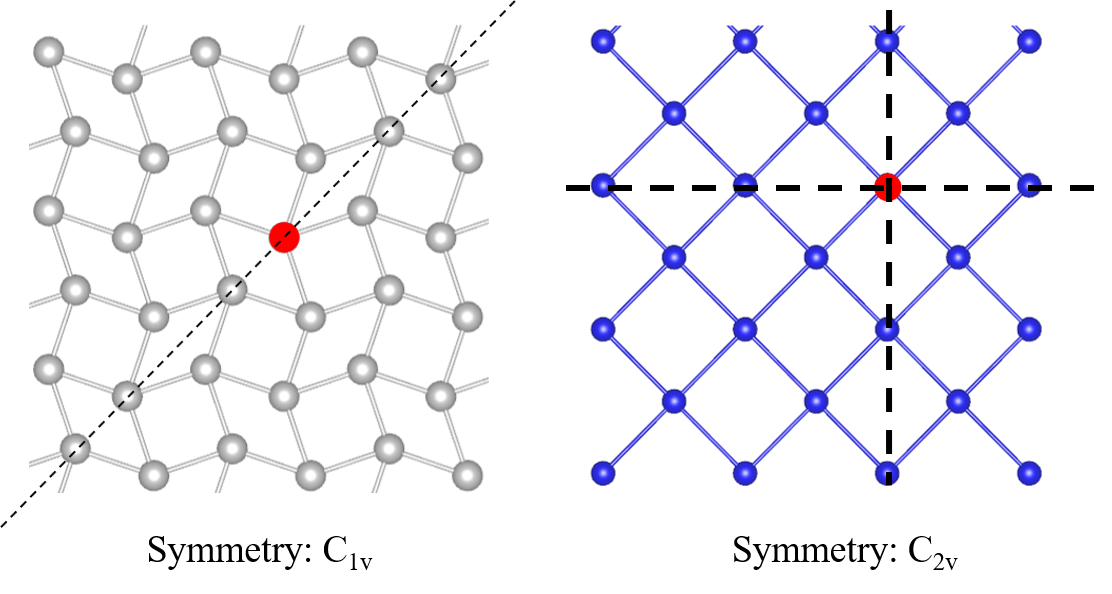
\includegraphics[width=\textwidth]{Ch4_symmetry.png}
	\caption{In plane lattice symmetry, left: Sn layer, right: Pt layer}
	\label{fig:ch4_symmetry}
\end{figure}

\subsection{Defect Statistics}

\subsubsection{Statistical Framework}
Defect density is a direct metric to evaluate the level of lattice perfection of a system. To achieve a reliable defect density and their associated undertainties, we used a statistical framework grounded in binomial and Poisson distribution principles, and justify its applicability to our experimental observations.
\par Our analysis of defect densities in PtSn4 crystals commences with the consensus that that point defects emerge as a stochastic process\cite{rudolph_defect_2010},\cite{mosquera-lois_imperfections_2023}. Given the crystal lattice structure, defects can randomly occur at any site, rendering each occurrence an independent event. This randomness and independence are fundamental assumptions that underpin our methodological approach, it is justified by STM topography as mentioned in the later paragraph.  
\par In total, 3 types of Sn-site defects and 6 kinds of Pt defects are observed. Since each site can only be occupied by one defect, to individual types of defect, we can conceptualize each lattice site as a discrete trial within a binomial framework. A 'success' in this context was defined as the presence of this particular type of point defect at a given site, denoted by '1', while its absence was considered a 'reference event', denoted by '0'. This binary scheme facilitated the application of the binomial distribution to model the statistics of defect occurrences across the lattice.
\par Given the expansive scanning area corresponding to a vast number of lattice sites (trial), coupled with the markedly low probability of defect occurrence (success rate), our analysis necessitated an approximation to simplify computations and enhance analytical tractability. The 
binomial distribution converges to the Poisson distribution under these conditions of large trial numbers and a small success rate. This approximation is underpinned by established statistical criteria. When the number of trials (n) exceeds 100 and the success rate (p) is below 0.1, the Poisson distribution serves as an effective surrogate for the binomial distribution. 
\par In our specific case, with n on the order of $10^5$ and p ranging between $10^-3$ and $10^-5$, the mean of the Poisson distribution ($\lambda=n\cdot p$) falls between 1 and 100. These are the conditions where the Poisson approximation is not only justified but advantageous, facilitating a more streamlined analysis of defect densities.
\par The sparse and non-clustered distribution of defects, as revealed through Scanning Tunneling Microscopy (STM) topographies, provided empirical validation for our methodological choices. The lack of defect clustering corroborates the assumption of defect occurrences as independent events, likely driven by thermal activation rather than mechanical strain. Mechanical strain would predictably induce clustering or patterned distributions of defects due to stress relaxation dynamics within the crystal lattice.
\par The transition from a binomial to a Poisson framework is further justified by the nature of our observations and the computational efficacy it offers. The Poisson distribution, known for its applicability to rare events in large populations, aligns well with the characteristics of defect formation in PtSn4 crystals. This alignment not only simplifies the mathematical treatment of defect statistics but also enhances the interpretability of our findings.

\subsubsection{Defect counting}
Defect counting is one of the key components to this study. Before the labour work of manually counting the defects, it is important to sample our image pool to avoid bias and enhance statistical representativeness. There are a few principles I followed with image selection: 
\begin{itemize}
	\item 1. Use images with good and consistent tip conditions(here the standard is whether the tip can image atomic resolution), but images taken at different bias voltages are allowed. 
	\par Rationale: Defects images taken by consistent tip conditions will give a more consistent pattern and thus more robust counting.	
	\item 2. Avoid repetitive areas. 
	\par Rationale: Many of the images are take on the same area to gauge the tip conditions.
	\item 3. Choose big size images, here we use images of size bigger than 50nm by 50nm.
	\par Rationale: Smaller size images are usually taken to focus on object of interest, thus biased.  
\end{itemize}  
Just to give the reader a sense, we collected around 20000 topographic images in our study, after standard 1, we are left with around 3000 images, then we apply standard 2, we again eliminate about 80\% of the images, and with standard 3, we are left with in total 55 images, with 33 on HR sample and 22 on LR samples. However, with the statistical framework we established in last section, the areas covered by these images are still big enough for us to make statistically meaningful claim on defect density.

\subsubsection{Defect density}

\begin{table*}
		\renewcommand{\arraystretch}{1.5}  % Increased line separation
		\caption{Defect statistics of two samples of PtSn$_4$ grown at two different cooling rates: slow-cooled sample S1 (RRR~$>1000$) and fast-cooled sample S2 (RRR~$=200$).} \label{tab:table1}
		\begin{tabular}{ccccc}
			Defect & Symmetry & Category & $\rho A_{\text{S1}}$ (per unit cell) & $\rho A_{\text{S2}}$ (per unit cell) \\ 
			\hline
			Sn$_1$ (Croissant)\footnote{This kind of defect is believed to be non-intrinsic} & $C_{1v}$ & Sn site & $1.00(0.02) \times 10^{-3}$ & $3.50(0.03) \times 10^{-3}$ \\
			Sn$_2$ (Spearhead)$^{\text{a}}$ & $C_{1v}$ & Sn site & $1.46(0.02) \times 10^{-3}$ & $0.216(0.008) \times 10^{-3}$ \\
			Sn$_3$ (Crescent)$^{\text{a}}$ & C$_{1v}$ & Sn site & $1.545(0.007) \times 10^{-4}$ & $0.033(0.009) \times 10^{-4}$ \\
			\hline
			Pt$_1$ & $C_{2v}$ & Pt site & $2.9(0.5) \times 10^{-5}$ & $5.6(0.4) \times 10^{-5}$ \\
			Pt$_2$ & $C_{2v}$ & Pt site & $3.8(0.5) \times 10^{-5}$ & $5.4(0.4) \times 10^{-5}$ \\
			Pt$_3$ & $C_{2v}$ & Pt site & $1.7(0.3) \times 10^{-5}$ & $2.1(0.3) \times 10^{-5}$ \\
			Pt$_4$ & $C_{2v}$ & Pt site & $2.8(0.4) \times 10^{-5}$ & Not Observed \\
			Pt$_5$ & $C_{2v}$ & Pt site & Not Observed & $2.0(0.2) \times 10^{-5}$ \\
			Pt$_6$ & $C_{2v}$ & Pt site & Not Observed & $0.5(0.1) \times 10^{-5}$ \\
			\hline
			Sn$_{\text{total}}$ &  &  & $2.61(0.03) \times 10^{-3}$ & $3.72(0.03) \times 10^{-3}$ \\
			Pt$_1$+Pt$_2$+Pt$_3$ &  &  & $0.84(0.08) \times 10^{-4}$ & $1.31(0.06) \times 10^{-4}$ \\
			Pt$_{\text{total}}$ &  &  & $1.1(0.08) \times 10^{-4}$ & $1.56(0.07) \times 10^{-4}$ \\
		\end{tabular}
\end{table*}

\par Defect densities for each type are reported in Table~\ref{tab:table1}. defect densities are reported on both the highRRR and lowRRR sample. Pt site defects are significantly rarer than Sn site defects, as discussed below. Of the 6 types of Pt-site defects, Pt$_{1}$,Pt$_{2}$ and Pt$_{3}$ were observed in both samples. All Pt site defects are in the range of 10--50 ppm, and of the three types present in both high and lower RRR samples, all increase in the fast-cooled lower RRR sample. The overall density of Pt site defects increases for the lower RRR sample, consistent with expectations from the increased low-temperature resistivity originating from point defect scatterers.

\par Defects residing on the Sn site are more prevalent in both samples, having densities that are between one and two orders of magnitude larger than the Pt site defects. However, the analysis is confounded by sensitivity to surface effects. Although significant increases in defects over time due to the adsorption of contaminants were not observed, other extrinsic variability appears to significantly influence the total Sn site defect density. In particular, the Sn$_1$ (croissant) defect is readily induced by the tip through voltage pulses or prolonged high voltage, and these defects have been observed to move and even annihilate, leading us to suspect these defects correspond to a Frenkel pair (a Sn adatom-Sn vacancy pair). The Sn$_2$ and Sn$_3$ defects anomalously decrease in the fast-cooled (lower RRR) sample, contrary to expectations from the transport measurements. We suspect these correspond to vacancies and/or adatoms that arise during cleaving, as the Sn surface is easily disturbed. With these extrinsic factors in mind contributing to the total observed defect density, we can only place an upper limit on the number of scattering sites. However, we note that as no new defect types appear, and all are sensitive to disorder reorganization of atoms, we do not observe any Sn-site defects corresponding to chemical substitutions - in other words, no other atoms are present on the Sn sites. While intrinsic Sn site defects are surely present, they are dominated by extrinsic ones, we will therefore focus more on the Pt site defects.

\par Having established that the Pt site defects provide a more reliable indicator of the intrinsic defect concentration, we can next examine the differences between samples S1 (higher RRR) and S2 (lower RRR). Pt$_1$, as the dominant intrinsic defect, doubled in the lower RRR sample, and the Pt$_2$ defect also has a sizable increase in the low RRR sample. And Pt$_3$ does not have a notable change in the density. Taken in aggregate the increase in defects corresponds to a $1.5\times$ larger concentration of Pt site defects in S2 with a lower RRR as compared to S1 with a higher RRR.  The increase in intrinsic defect densities is aligned with the decrease in the low-temperature resistivity across the two samples. However, naively, we would expect a linear correlation between defect concentration and residual resistivity due to electron-defect scattering. The observed increase of $1.5\times$ in the Pt site defects described here fails to account for the $5\times$ decrease in the RRR value for S2 as compared to S1. We therefore conclude that, although the Sn site defects are dramatically obscured by the non-intrinsic effects described above, they must account for the majority of increased scattering centers. 

\subsection{Non-Intrinsic Defects in PtSn$_4$} \textcolor{red}{In Appendix?}

\begin{figure}
	\centering
	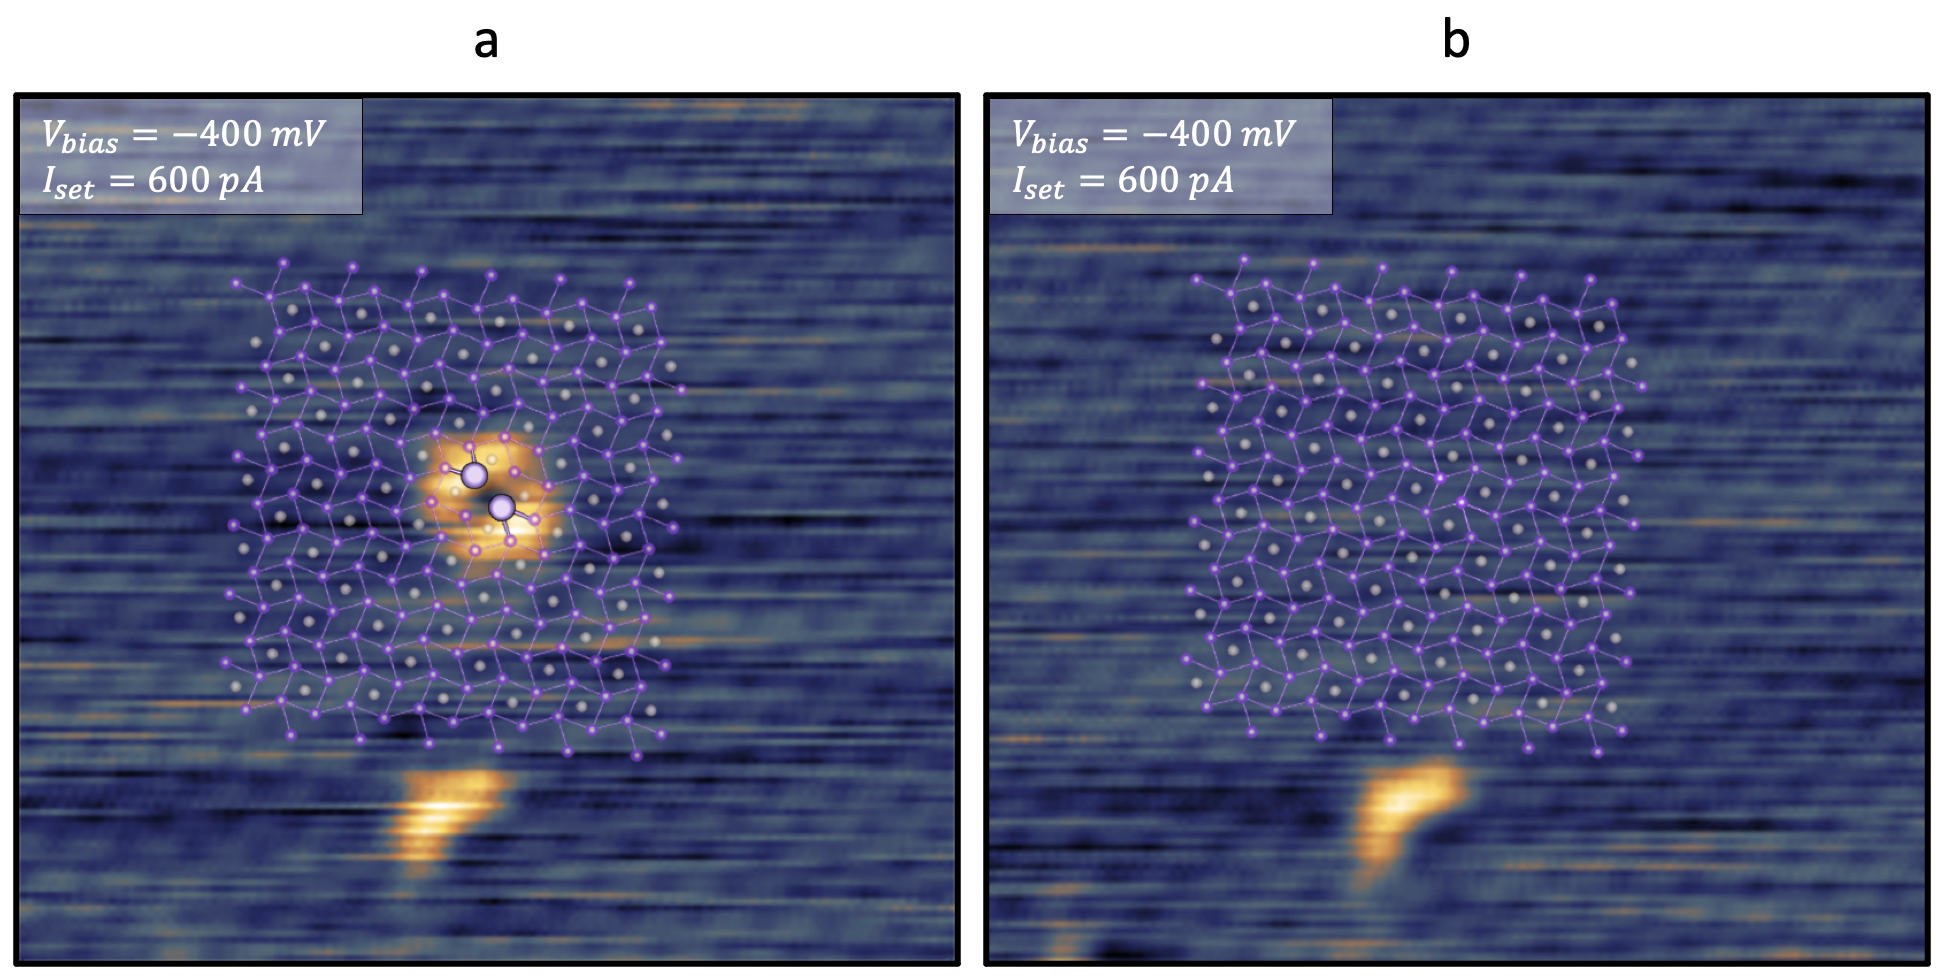
\includegraphics[width=0.8\textwidth]{Ch4_croissant.png}
	\caption{Two Sn$_1$ defect annihilation, indicating the origin of Sn$_1$ defects being from Frankel pairs}
	\label{fig:Ch4_croissantannihilation}
\end{figure}

\begin{figure}
	\centering
	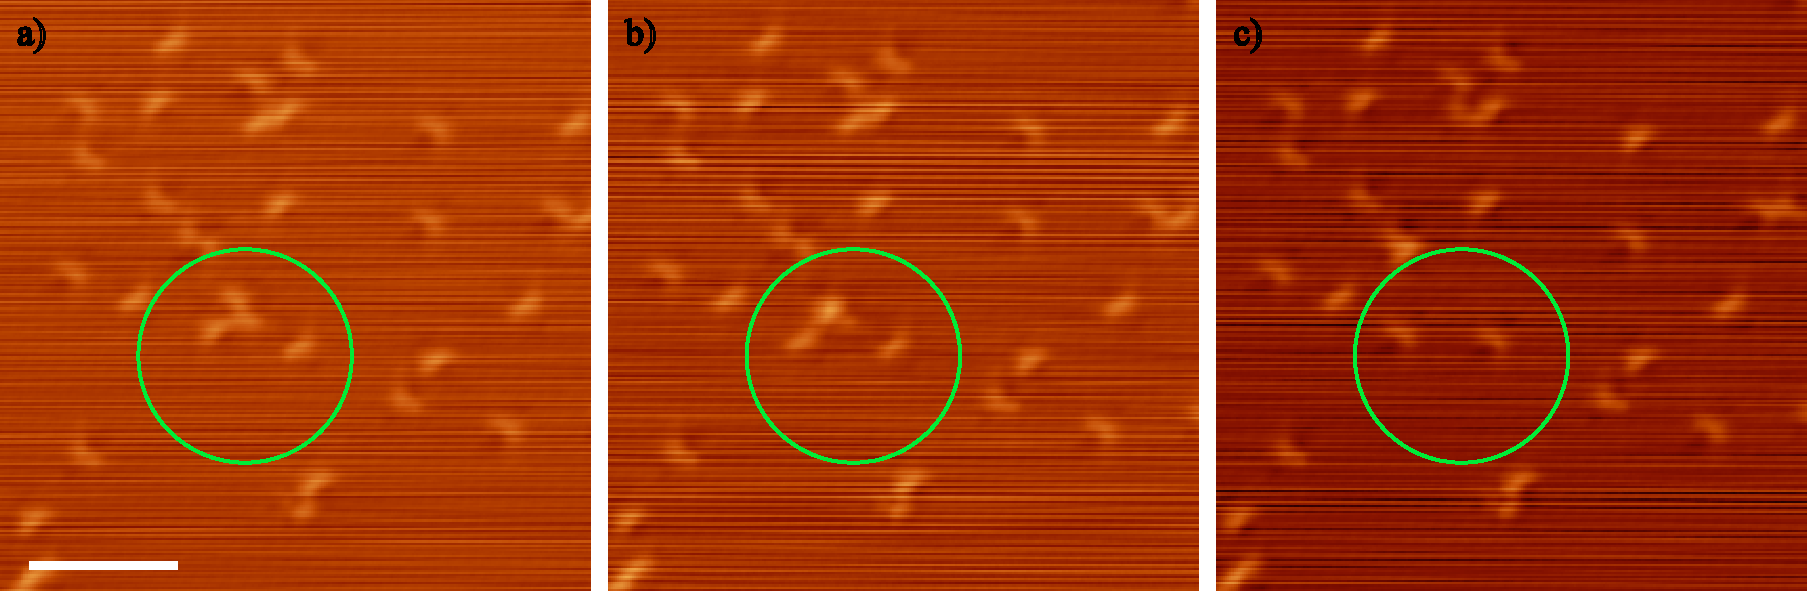
\includegraphics[width=0.8\textwidth]{Ch4_rotationcroissant.pdf}
	\caption{Sn$_1$ defect under consecutive scans, rotations and annihilation were found in the green circle.}
	\label{fig:Ch4_rotationcroissant}
\end{figure}

\par In our experiment, we have observed that the Sn1 defect, located at the Sn-site, is highly mobile under conditions of high scanning biases (exceeding 600mV). Notably, rotation of this defect is consistently observed in consecutive scans, example given in \ref{fig:Ch4_rotationcroissant}, and instances of annihilation between two Sn1 defects have also been documented, as shown in \ref{fig:Ch4_croissantannihilation} and \ref{fig:Ch4_rotationcroissant} b) to c). These events demonstrate the ability to both create and annihilate defects during scanning. This behavior also suggests that the origin of the Sn1 defect could be a Frankel pair on the Sn site. %could elaborate more on the origin of Sn1 defect. 
%todo: prepare figure on the population over different macroscopic spots. 
\par Moreover, the density of Sn1 defects varies significantly across different macroscopic locations on the crystal, as evidenced in STM observations (e.g., figure X). This variation, with density differences exceeding fiftyfold among explored locations, suggests that different cleaving planes may influence the introduction of Sn1 defects. Such spatial dependence supports the hypothesis that Sn1 defects could also be introduced during the cleaving process, reinforcing their classification as non-intrinsic.

\par While there is no direct evidence to suggest that Sn2 and Sn3 defects are non-intrinsic, the observed decrease in their densities from samples with higher residual resistivity ratio (RRR) to those with lower RRR supports the likelihood of these defects also being non-intrinsic. This variation could be indicative of differences in crystal order influenced by experimental conditions rather than intrinsic material properties.

\par In conclusion, while the intrinsic qualities of PtSn$_4$ are well-represented in STM studies, the influence of experimental techniques such as cleaving and scanning under bias voltage introduces a variety of non-intrinsic defects. However, it is worth noting that despite the ability to introduce these defects via experimental manipulations, these defects can still intrinsically exist in bulk samples, making the studies around these defects relevant. 

\section{discussion}
%todo: to write this section after ch.3 is finished
\par This section need to be written after the intro for PtSn4. ie Ch.2. 

\par This reasoning is consistent with both the numerically larger concentration of Sn atoms relative to Pt and the significantly reduced cost to form a Sn site vacancy as compared to a Pt Site vacancy as determined by DFT. Nonetheless, the dramatically small number of Pt site defects, where the occurrence of intrinsic defect is as rare as 1 in 10,000 unit cells, is good evidence that crystalline perfection is the underlying cause for the long mean free paths and hence the high RRRs observed in PtSn$_4$. 

\chapter{Quasiparticle Interference (QPI)}
%todo: to write the abstract of this chapter after finishing this chapter
%todo: to standardize the vector form in this chapter 
\section{Introduction to Quasiparticle}
A Quasiparticle is any long-lived, well-defined excitation in a system that behaves like a particle, it is a semi-classical term used to describe particle interactions in terms of renormalized single-particle excitation. In Fermionic systems, it corresponds to a sharp peak in the spectra function: 
	\[
	A(\mathbf{k}, \omega) = -\frac{1}{\pi} \frac{\operatorname{Im} \Sigma(\mathbf{k}, \omega)}{(\omega - \tilde{E}_{\mathbf{k}})^2 + [\operatorname{Im} \Sigma(\mathbf{k}, \omega)]^2},
	\]

This section aims to introduce the concept of a quasiparticle, first through a historical overview of the development of quasiparticle theory, relevant languages and terms will be established, as well as the assumptions and limitations of the theory; then we illustrate the concept quantitatively through a microscopic theory of landau quasiparticles. 

\subsection{The historical overview}
The development of a quasiparticle model for Fermionic systems started in 1940s, when Sommerfeld and Bethe\cite{SommerfeldBethe1933} developed a model for a non-interacting electron gas, also known as the 'Fermi gas', in which a series of important terms are introduced. Consider a system made of non-interacting electrons with momentum $k$ and spin $\sigma = 1/2$, which is in touch with an electron reservoir with chemical potential $\mu$. The occupation number follows the Fermi-Dirac distribution $n_{k,\sigma}=1/(1+e^{(k^2/(2m)-\mu)/T}))$. At $T=0$, the occupation thus has a sharp boundary known as the Fermi surface, in the momentum space confined by the Fermi wave number $k_f$, and the energy defined by the Fermi surface is called the Fermi energy. At non-zero temperature, electrons at the Fermi energy will start to be excited above the Fermi energy; this excitation can also be described in second-quantization by the creation of a quasiparticle with energy: $\epsilon_{k,sigma} = k^2/2m - \mu$. 

Sommerfeld's theory of the electron gas worked quite well in standard metallic systems, but the success was unexpected, as the model neglected the Coulomb interaction between electrons. In a metallic system where the electron separation is in the order of the lattice spacing, the Coulomb interaction is in the order of eV, which is much larger than other energy scales, say, the thermal excitation considered in the electron gas mode. 

In the late 1960s, Landau raised a theory of the Fermi liquid with a series of foundational papers\cite{Landau1956}\cite{Landau1957} to address that even in the presence of interactions, we can find fermionic excitations in these many-body systems, and describe these excitations with what is known as the Landau quasiparticles. By adding a time-variant interaction term, defined by time constant $\zeta$ to the non-interactive system, and constructing the system Hamiltonian as
\begin{equation}\label{adiabatic}
	H_{\zeta} = H_0 + H_{\text{int}} e^{-\zeta t}, \quad t > 0,
\end{equation}

By the principle of adiabatic continuity, Landau is able to bridge between the states of interactive and non-interactive systems. Consequently, the states describing the interactive system can now be reduced to states in the non-interactive system with the same quantum numbers $k, \sigma$. More specifically, as quoted from \textit{What is a Quasi-Particle?} by J.R.Schrieffer, "these many-body states are well characterized in terms of a set of elementary excitations, called quasi-particles, which for the interacting system play the same role as the excited electrons(above the Fermi surface) and the excited holes(below the Fermi surface) in the Independent-particle approximation(IPA)." 

Landau's quasiparticle is an extremely useful concept in computing the screening and the transport properties of an electron-gas-like system. However, we should emphasize that the theory is only valid with several assumptions:

For an adiabatic procedure to hold, time scale $\zeta$ in Equation \ref{adiabatic} should be bounded by two conditions: 1. rate of evolution should be small compared to the energy of the state: $\zeta << \epsilon_{k,\sigma}$, 2. the final bound state remains the same as the initial one, meaning the lifetime $\tau_{life}$ of the bound state should be long enough: $\tau_{life} >> \zeta^{-1}$. Therefore, $\zeta$ should suits: 
\begin{equation}
	\tau_{life}^{-1} << \zeta << \epsilon_{k,\sigma},
\end{equation}
since typical excited energy is in the order of temperature, and the lifetime is inversely proportional to $T^2$, we can also write:
\begin{equation}
	T^2 << \zeta << k_B T,
\end{equation}
This requirement can be satisfied at a range of low temperature. Later we will also see that the requirements also extend to the energy level of the states, since the quasiparticle lifetime decreases as energies deviate from the Fermi energy. 
%todo: can refer to the chapter where we talk about the lifetime decay with simulation. 
%Therefore, Landau's theory of Fermi liquid postulated that an interacting fermionic system can we mapped adiabatically to a non-interacting Fermi gas, with long-lived quasiparticle that shares the same quantum numbers near the Fermi surface. 
In electronic systems, the theory works in a regime with weak to moderate electron-electron correlations at sufficiently low temperatures, and thus, it succeeds in explaining the properties of simple and noble metals. For more detailed reading regarding the theory, the textbooks of Pines and Nozieres\cite{nozieresTheoryQuantumLiquids2018a} and Nozieres \cite{nozieresDerivationLandauTheory1962} offer derivations and in-depth discussions. 

Landau's theory failed to address more involved systems; however, based on the theory, scientists formulated a more generalized concept of quasiparticles through the lens of Green's function scheme of many-body theory. There have been many extensions and refinements of the quasiparticle theory throughout history; the meaning of quasiparticles and the corresponding regime where this can be applied varied drastically. Here, I would like to provide a rough list of those theories chronologically and give brief notes on them:
\begin{itemize}
	\item\textbf{Hartree-Fock Approximation (HF)} (1930s):
	HF approximation is not an extension of Fermi liquid theory but it is the first step beyond a purely free-electron model, and it lays groundwork for diagrammatic expansions \cite{fockNaeherungsmethodeZurLoesung1930}, \cite{slaterNoteHartreesMethod1930}.
	
	\item\textbf{Random Phase Approximation(RPA)} (1950s): 
	RPA extends the theory to moderate correlations where long-range screening is crucial, including dynamical screening. It successfully explains quasiparticle dispersion like plasmon dispersion and optical properties in metals and semiconductors \cite{bohmCollectiveDescriptionElectron1951}, \cite{nozieresCorrelationEnergyFree1958}.
	
	\item \textbf{BCS theory} (1957):
	BCS theory of superconductivity established a microscopic explanation for the superconducting phase transition, which was initially described macroscopically by Ginzburg–Landau theory as a second-order phase transition with an order parameter $\Delta$. For $T>T_c$, one can describe the normal state low temperature excitations with landau quasiparticles, these quasiparticles are unstable approaching $T_c$ with a weak attractive interaction, as shown by Cooper\cite{cooperBoundElectronPairs1956}, and forms Copper pairs that breaks gauge symmetry and lead to superconducting phase. In the superconducting phase, the low energy excitations can be described by Bogoliubov quasiparticles. Since the excitations are gapped by a pairing gap $\Delta_k$; Bogoliubov quasiparticles have a finite energy and therefore are well defined and long-living in a clean superconductor \cite{bardeenTheorySuperconductivity1957},\cite{tinkhamIntroductionSuperconductivity2004}.
 
	\item\textbf{Gutzwiller(GW) Approximation} (1965):
	GW approximation provided a more accurate approximation than RPA and can be implemented to stronger correlated systems \cite{hedinNewMethodCalculating1965}, \cite{aryasetiawanGWMethod1998}.
	
	\item\textbf{Dynamical Mean-Field Theory(DMFT)} (1990s):
	DMFT was developed via a non-perturbative approach, this allows it to extend the concept of quasiparticles to account for strong local correlations in systems like transition metal oxides and f-electron materials. Although it kept the concpt of quasiparticles, it showed that they failed near Mott transitions when electron-electron interaction is large enough \cite{metznerCorrelatedLatticeFermions1989}, \cite{georgesDynamicalMeanfieldTheory1996}.
	
	\item\textbf{GW + DMFT} (2000s):
	This combined method took the best of GW(dynamic and non-local screening) with DMFT(local, but exact correlation), making it suitable for systems with moderate to strong correlation as well as significant screening effects, like heavy fermion compounds \cite{biermannFirstprinciplesApproachElectronic2003}.
\end{itemize}

A more detailed history of the development of the quasiparticle theory and its more recent application into systems like topological materials can be found in Peter et al.\cite{wolfleQuasiparticlesCondensedMatter2018}. 

\subsection{Microscopic Theory of Quasiparticles}
Landau quasiparticles are added to a system with the creation of the excitations, therefore, we need to look at the retarted Green's function $G^R$ as it measures the density of states for adding particles, and thus a system's response to creating or annihilating a single fermion at a given state. We consider the one-particle retarded Green's function: 
\begin{equation}\label{retardedgreen}
	G^R_{k \sigma, \omega} = \frac{1}{\omega -\epsilon_k - \Sigma^R(k \sigma, \omega)},
\end{equation}
where $\epsilon_k= \frac{k^2}{2m-\mu}$ is the free electron energy with respect to the chemical potential $\mu$, and $\Sigma^R_{k \sigma, \omega}$ is the retarded self-energy that is irreducible in diagrammatic expansion. 

We then expand the self-energy into real and imaginary parts, the effective single-electron energy is $\epsilon'_{k} = \epsilon_k + \operatorname{Re}\Sigma^R(k,\omega)$. We can then define the renormalized Fermi momentum $k^*_{F}$ as $\epsilon'_{\tilde{k_{F}}} = 0$. Then we expand $G^R_{k, \omega}$ around $k = k^*_{F}$ and get: 

\begin{equation}
\label{gr_full}
G^{R}(\mathbf{k}, \omega) \approx Z \left[ \omega - \epsilon^*_{\mathbf{k}} + i \Gamma_{\mathbf{k}} \right]^{-1}
\end{equation}
where
\begin{align} 
	Z^{-1} &= 1 - \left. \frac{\partial}{\partial \omega} \, \mathrm{Re} \, \Sigma (k^*_{F}, \omega) \right|_{\omega = 0}, 
	\\ 
	\label{eq2}
	\epsilon^*_{\mathbf{k}} &= (k - k^*_{F}) Z \left. \frac{\partial}{\partial k} \left( \epsilon_{\mathbf{k}} + \mathrm{Re} \, \Sigma ({k}, 0) \right) \right|_{k = k^*_{F}}, \\ 
	\label{gamma}
	\Gamma_{\mathbf{k}} &= Z \mathrm{Im} \Sigma^{R}({k}, 0) 
\end{align}

\noindent here, $\epsilon^*_{\mathbf{k}}$ is the renoramlized energy, $\Gamma_{\mathbf{k}}$ is the relaxation rate which is inverse proportional to the quasiparticle lifetime $\tau_{life}$, and $Z$ is called the weight factor of qausiparticles. We can further parameterize the renormalized energy with effective mass $m^*$: 
\begin{equation}\label{energy}
	\epsilon^*_{\mathbf{k}} = \frac{k^*_F(k-k^*_F)}{m^*}
\end{equation}
We can then plug \ref{energy} to \ref{eq2} and get: 

\begin{equation}
	\frac{m}{m^*} = Z(1 + \frac{m}{k^*_F}\frac{\partial}{\partial k}\operatorname{Re}\Sigma(k,0)|_{k = k^*_{F}})
\end{equation}

We can see that by introducing the retarded self-energy that encodes the interaction effects on single particles, we can describe the system near the modified Fermi momentum with quasiparticles. These quasiparticles are characterized by an effective mass $m^*$ that is dictated by the real part of self-energy and a lifetime $\tau_{life}$ that is inversely proportional to the imaginary part of self-energy. Providing the imaginary part of self-energy very small, we have long lived quasiparticles, and hence we can write the Spectral function from \ref{gr_full}:
\begin{equation}
	\label{eq.akw}
	A(\textbf{k},\omega) = -2\operatorname{Im}G^R(\textbf{k}, \omega) 
	\approx 2\pi Z\delta(\omega-\epsilon^*_\textbf{k}) 
\end{equation}

This indicate a sharp peak at $\omega=\epsilon^*_\textbf{k}$, thus resembles the spectral function of a Fermi gas, and the pole is what we call the quasiparticle in the Fermi liquid theory. However, we can see that \ref{eq.akw} does not fulfill the normalization rule: 
\begin{equation}
	\int_{-\infty}^{+\infty} \frac{d\omega}{2\pi} A(\textbf{k},\omega) = 1, 
\end{equation}

we need to incorporate another term $A'(\textbf{k},\omega)$ into $ A(\textbf{k},\omega)$ to that has an integrated wight given by 1-Z, giving us: 
\begin{equation}
	\label{eq.akw}
	A(\textbf{k},\omega) = 2\pi Z\delta(\omega-\epsilon^*_\textbf{k}) + A'(\textbf{k},\omega)
\end{equation}
Fig. \ref{fig:ch5_spect} \cite{bruusManyBodyQuantum2004} illustrates this effect, and that term $A'(\textbf{k},\omega)$ captures the remaining excitations other than the well defined quasiparticle pole. 

\begin{figure}
	\centering
	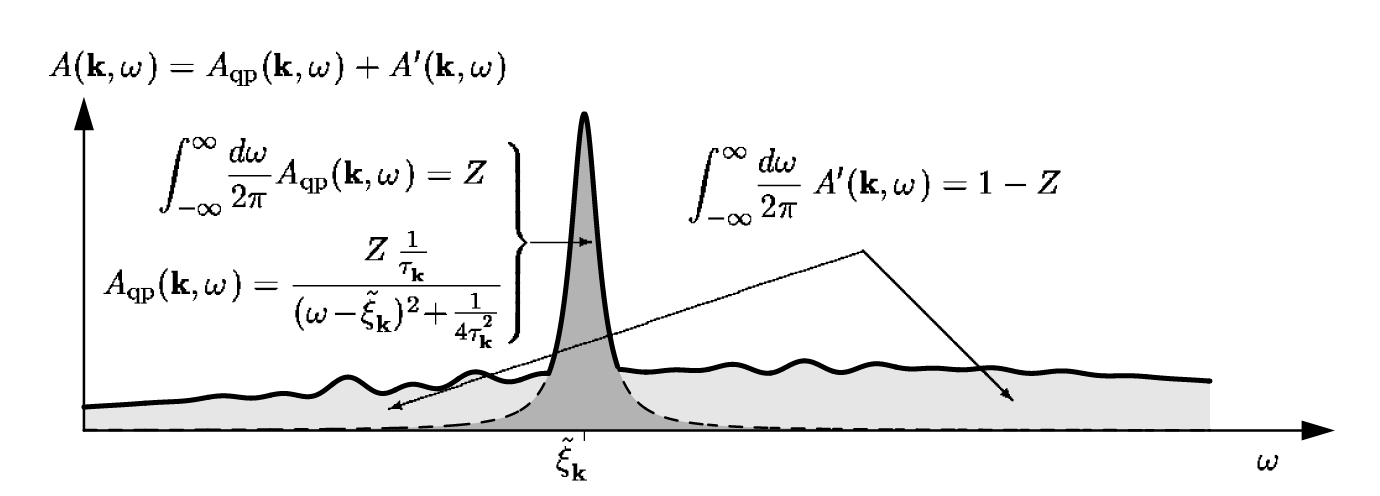
\includegraphics[width=\textwidth]{Ch5_spectralfunciton.png}
	\caption{The spectral function $A(\textbf{k},\omega)$ that includes the quasiparticle peak and the background function $A'(\textbf{k},\omega)$ stemming from other types of excitation}
	\label{fig:ch5_spect}
\end{figure}

\section{Introduction to Quasiparticle Interference}

In the Fermi liquid theory, an interactive many-particle system is modeled by a renormalized single-particle system, with quasiparticles capturing the excitations near the renormalized Fermi level. These quasiparticles are long-living and carry the same quantum numbers $(\textbf{k}, \sigma)$ as the bare particles. The non-infinite lifetime corresponds to the weakly interactive nature of the quasiparticles; interactions involved quasiparticles include quasiparticles-quasiparticle interaction of the same kind, e.g. the phonon-phonon interaction in anharmonic lattices \cite{kimExploringAnharmonicLattice2023}; quasiparticles of a different kind, e.g. the exciton-phonon coupling in ZnO \cite{mendelsbergPhotoluminescenceExcitonphononCoupling2011}; or interact with other elements like impurities on the lattices \cite{avrahamQuasiparticleInterferenceStudies2018}. 

One can utilize the interactions that involve quasiparticles as a channel to explore properties of matters. In particular, when it comes to single-particle properties, or more specifically, probing the spectral function $A(\textbf{k},\omega)$, the tunneling experiment is at a unique position because of its ability to both inject and remove an electron into and out of a many-body system.  

As \ac{STM} combines the ability to resolve both the spatial and energy dimensions of the electron density of states; We can perform a powerful measurement call Quasiparticle Interference measurement, or \ac{QPI} measurement. This section aims to introduce \ac{QPI} measurement, exploring both its theoretical foundation as well as the experimental details. We will then point out challenges of performing and interpreting a "good" \ac{QPI} measurement. This should give a direct motivation for our next chapter, which introduced a method that we use to mitigate some of the challenges. 

\subsection{Terminology}
To set stage for the discussion in this chapter, we must make distinctions between the following terminologies: 
\begin{itemize}
	\item QPI: The interference between the incoming quasiparticle and the outgoing quasiparticle in a scattering event between quasiparticles and lattice imperfections.  
	\item QPI pattern: an interference pattern that can be observed by \ac{STM} on the surface of the material.
	\item QPI measurement: a measurement that measures the QPI patterns presented in systems that intrinsically host QPI. This hinted an assumption that the tunneling experiment did not induce the scattering, but act as a mere observer of this phenomenon.
\end{itemize}
%We should note that STM is not the only tool that can perform QPI measurement. In fact, interference of quasiparticles are reported across a wide literature in different systems using different techniques. For example,
%todo: to wirte different examples here, template as X used Y technique to detect G quasiparticle Interference pattern in Z system.: ranging from crystalline excitation like phonon in Si phononic crystals \cite{maldovan_phonon_2015}, electronic excitation like Bogoliubov quasiparticle in superconductors interference strongly\cite{homan_search_nodate}
I will then elaborate what these terms mean in the context of an STM study, and to reduce redundancy, in the following writing, QPI, QPI pattern and QPI measurement will be referred specifically to STM studies.

\subsection{QPI measurement in STM}
%todo: to plot a standard grid and its FFT here.
Understanding QPI pattern is the first step to understand QPI measurement. QPI pattern is the modulation of \ac{LDOS} due to quasiparticle-impurity scattering. The modulated \ac{LDOS} provides direct insight on the quasiparticle band structure. Imagine an ideal metal with no crystal imperfection; we know that the Landau quasiparticle has an eigenstate in real space described by a Bloch wavefunction: 

\begin{equation}
\psi(\mathbf{r}) = e^{i \mathbf{k} \cdot \mathbf{r}} u(\mathbf{r})
\label{eq:bloch}
\end{equation} 
where $k$ is the crystal momentum of the quasiparticle. And the electron \ac{LDOS} can be written as  
\begin{equation}
\text{LDOS}(E, \vec{r}) \propto \sum_k |\Psi_k(\vec{r})|^2 \delta(E - \varepsilon(k))
\label{eq:ldos}
\end{equation}

where  $\epsilon(k)$ is the renormalized energy dispersion of the Bloch state for different $\vec{k}$; Remark: from now on all the renormalized energy will be write directly as $\epsilon(k)$ unless otherwise mentioned. And if we plug Equation (\ref{eq:bloch}) into Equation (\ref{eq:ldos}), we see that $\text{LDOS}$ is translationally invariant at all Bravais-lattice-equivalent points. Thus why in ideal case, real space imaging technique like \ac{STM}, can not be used to measure $\epsilon(k)$. 

However, crystal imperfections as discussed in Ch.4 can help us introduce a momentum texture to the $\text{LDOS}(E, \vec{r})$. In low temperature STM, where the phonon modes and other excitation are rare or absent, lattice imperfections such as point defects can cause elastic scattering which mixes electronic eigenstates at different $\vec{k}$ but at the same energy, the interference between the incoming and outgoing wave forms a "standing wave" that act as a real space modulation in $\text{LDOS}(E)$ described as a impurity-induced Friedel oscillation\cite{benaFriedelOscillationsDecoding2016}. This spatial modulation in $\text{LDOS}$ is the QPI pattern that we refer to in STM studies. We can perform \ac{STS} measurement on the region that presents this QPI pattern, then perform Fourier transformation to the STS, we can also view this QPI pattern in the momentum space, the q-space QPI pattern is directly related to the quasiparticle band strucutre. This whole process of detecting QPI pattern and analyze it in momentum space is what we call a QPI measurement. 

We will quantitatively showcase this \ac{LDOS} modulation with a simulation on a toy model in the following section. 

%\begin{figure}
%	\centering
%	\includegraphics[width=0.5\textwidth]{example-image-a} % Replace with your image file
%	\caption{Friedel oscillation and QPI}
%	\label{fig:example}
%\end{figure}

\subsection{LDOS modulation simulation on a square lattice}

As mentioned in last section \ac{QPI} measurement is achieved by taking spectroscopy measurements on a real-space region that presents QPI pattern; As \ac{STM} spectroscopy probes the \ac{LDOS}, We must therefore, understand the origin of \ac{QPI} pattern and how it modifies \ac{LDOS}. Here, I present an investigation into the \ac{LDOS} modulation caused by point defects on a square lattice, this textbook exercise is inspired by work from Cheung et al \cite{cheungDictionaryLearningFouriertransform2020}.

\subsubsection{Theory}
We first consider a square lattice with lattice constant $a$, and model it through the single-electron Tight-Binding model considering only nearest-neighbor hopping. This hopping is characterized with a fixed negative number $t$ named hopping-parameter. We then place $N_d$ number of defects onto different lattice sites as a perturbation to the \ac{TB} Hamiltonian $H_0$. The total Hamiltonian can then be written as: 
$\hat{H} = \hat{H}_0 + \hat{H}_d$. $\hat{H}_d$ can be written as: 
\[
\hat{H}_d = \sum_{\alpha=1}^{N_d} E_\alpha \lvert \alpha \rangle \langle \alpha \rvert,
\] 
where $\alpha$ enumerates $\alpha^{th}$ defect located at $x_\alpha$, with energy $E_{\alpha}$ much smaller than hopping parameter $t$, we then write the \ac{TB} Hamiltonian and transfer it into momentum space:
\begin{align}
\hat{H}_0 = E_0 -t \sum_{j,\tau} (c_j^{+} c_{j+\tau} + c_{j+\tau}^{+} c_j) \label{h0_real} \\
\hat{H}_0 = E_0 -\sum_{k} \epsilon_k c_k^{+} c_k \label{h0_k} \\
\epsilon_k = -2t(cos(k_x a)+cos(k_y a)) \label{E_k}
\end{align}
Now we consider our measurable \ac{LDOS} $\rho(\mathbf{x},\omega)$:
\begin{equation}
\rho(\mathbf{x},\omega) = \rho^{0}(\mathbf{x},\omega) - \frac{1}{\pi} \operatorname{Im} \left[ \langle \mathbf{x} | \hat{G}_0 \hat{T} \hat{G}_0 |\mathbf{x} \rangle \right],
\label{ldos}
\end{equation}
where $\hat{G}_0$ and $\hat{T}$ are the \ac{BLGF} and the scattering T-matrix, respectively, according to the pertubative scattering theory. Since we are interested in the modulation of \ac{LDOS} caused by the defects, our actual observable is $\delta \rho(\mathbf{x}, \omega) \equiv \rho(\mathbf{x}, \omega) - \rho^{(0)}(\mathbf{x}, \omega)
$, which is the second term in Equation (\ref{ldos}).
To start, we need to compute the matrix element of \ac{BLGF} $G_0(\mathbf{x},\mathbf{x'},\omega)$:
\begin{align}
	G_0(\mathbf{x},\mathbf{x}';\omega) &= \langle \mathbf{x} | \hat{G}_0(\omega) | \mathbf{x}' \rangle, \\
\end{align}
where
\begin{align}
	\hat{G}_0(\omega) &= \int_{\text{BZ}} \mathrm{d}\mathbf{k} \, \frac{1}{\omega - \hat{H}_0} \lvert \mathbf{k} \rangle \langle \mathbf{k} \rvert \nonumber \\ 
	&= \int_{\text{BZ}} \mathrm{d}\mathbf{k} \, \frac{1}{\omega - E_\mathbf{k}} \lvert \mathbf{k} \rangle \langle \mathbf{k} \rvert,
\end{align}
where we have $\omega= \omega + i\epsilon$ to indicate the retarded Green's function and to capture the analytic continuation. Then we remind ourselves that in 2D, $\langle \mathbf{k}|\mathbf{x} \rangle = (\frac{1}{\sqrt{2\pi}})^2 e^{-i\mathbf{k}\mathbf{x}}$, and plug the energy dispersion Equation (\ref{E_k}) in, we get: 
\begin{align}
	G_0(\mathbf{x}, \mathbf{x}') = 
	\frac{1}{(2\pi)^2} \frac{1}{2t} 
	\int_{\text{BZ}} \mathrm{d}\mathbf{k} \, 
	\frac{e^{i k_1 (x_1 - x_1')} e^{i k_2 (x_2 - x_2')}}{b + \left( \cos(k_1 a) + \cos(k_2 a) \right)}. 
\end{align}
where $b \equiv \frac{\omega+ i\epsilon-E_0}{2t}$ is a dimensionless parameter, the $\i\epsilon$ is used to defined the retarded green's function by creating a pole in the complex plane, it also produces a better analytical continuation. we can then define a normalized position deviation $s_j \equiv \frac{1}{a}(x_j-x_j')$ and further reduced the matrix element to its final form: 
\begin{align}
	G_0(\mathbf{x}, \mathbf{x}') = 
	\frac{1}{(2\pi)^2} \frac{1}{2t a^2} 4 \, I_{\text{sq}} 
	\left( \frac{x_1 - x_1'}{a}, \frac{x_2 - x_2'}{a}, b \right) \label{blgf},
\end{align}
where
\begin{align}
	I_{\text{sq}}(s_1, s_2, b) \equiv 
	\int_0^\pi \int_0^\pi \mathrm{d}\phi_1 \, \mathrm{d}\phi_2 \, 
	\frac{\cos(s_1 \phi_1) \cos(s_2 \phi_2)}{b + \cos\phi_1 +b  \cos\phi_2} \label{Isq}.
\end{align}
Note that in the actual numerical calculation, the integral will be evaluated on an n by n grid of k-points.  
Now we proceed to compute the matrix element of T-matrix, we know that: 
\begin{equation}
	\hat{T} = \hat{H_d} (\hat{I} - \hat{G_0}\hat{H_d})^{-1}.
\end{equation} 
And for locations $x_\alpha$, $x_\beta$ on defect sites $\alpha$ and $\beta$, we have: 
\begin{align}
	T_{\alpha\beta} &= \langle \alpha|\hat{H_d} (\hat{I} - \hat{G_0}\hat{H_d})^{-1} | \beta\rangle \\
	&= E_\alpha(\langle \alpha|\hat{I}|\beta\rangle - \langle \alpha|\hat{G_0}\hat{H_d}|\beta \rangle)^{-1} \\
	&= E_\alpha(\delta_{\alpha \beta} - E_\beta G_0(\mathbf{x_\alpha},\mathbf{x_\beta}))^{-1} \label{T_matrix_ele}.
\end{align}
Now with both matrix elements of the \ac{BLGF} and T-matrix, we can finally express $\delta\rho(\mathbf{x},\omega)$ as 
\begin{align}
	\delta\rho(\mathbf{x},\omega) &= - \frac{1}{\pi} \operatorname{Im} \left[ \langle \mathbf{x} | \hat{G}_0 \hat{T} \hat{G}_0 | \mathbf{x} \rangle \right] \\
	&= -\frac{1}{\pi} \operatorname{Im} \left[\sum_{\alpha, \beta=1}^{N_{\text{d}}} G_0(\mathbf{x}, \mathbf{x}_\alpha) T_{\alpha, \beta} G_0(\mathbf{x}_\beta, \mathbf{x})\right]. \label{multi_defect_eq}
\end{align}
In single defect case, where $\mathbf{x_\alpha} = \mathbf{x_\beta} = \mathbf{x_d}$, we have: 
\begin{align}
	T(\mathbf{x_d},\omega) &= E_{\text{d}} \left( 1 - E_{\text{d}} G_0(\mathbf{x_d}, \mathbf{x_d}) \right)^{-1} \label{T_matrix_ele} \\
	&= \frac{1}{E_{\text{d}}^{-1} - G_0(\mathbf{x_d}, \mathbf{x_d}; \omega)},
\end{align}
and therefore: 
\begin{align}
	\delta\rho(\mathbf{x},\omega) &= - \frac{1}{\pi} \operatorname{Im}(\frac{G_0^2(\mathbf{x},\mathbf{x_d};\omega)}{E_d^{-1} - G_0(\mathbf{x_d},\mathbf{x_d};\omega)}) \label{singleldos}. 
\end{align}
And Equation (\ref{singleldos}) can be evaluated numerically with Equation (\ref{blgf}) and Equation (\ref{Isq}).

\subsubsection{Simulation result}
A repository for \ac{LDOS} simulation on the model described above is made and shared on this \hyperlink{https://github.com/Plswearpants/QPI_simulation}{github repository}

The setup of simulation is illustrated in \ref{fig:ch5_qpisim_demo}, a grid of $128x128$ in real space covering a $20x20$ lattice space indicated in orange dots. We can implant defects on different lattice sites, indicated in green dots. 

\begin{figure}
	\centering
	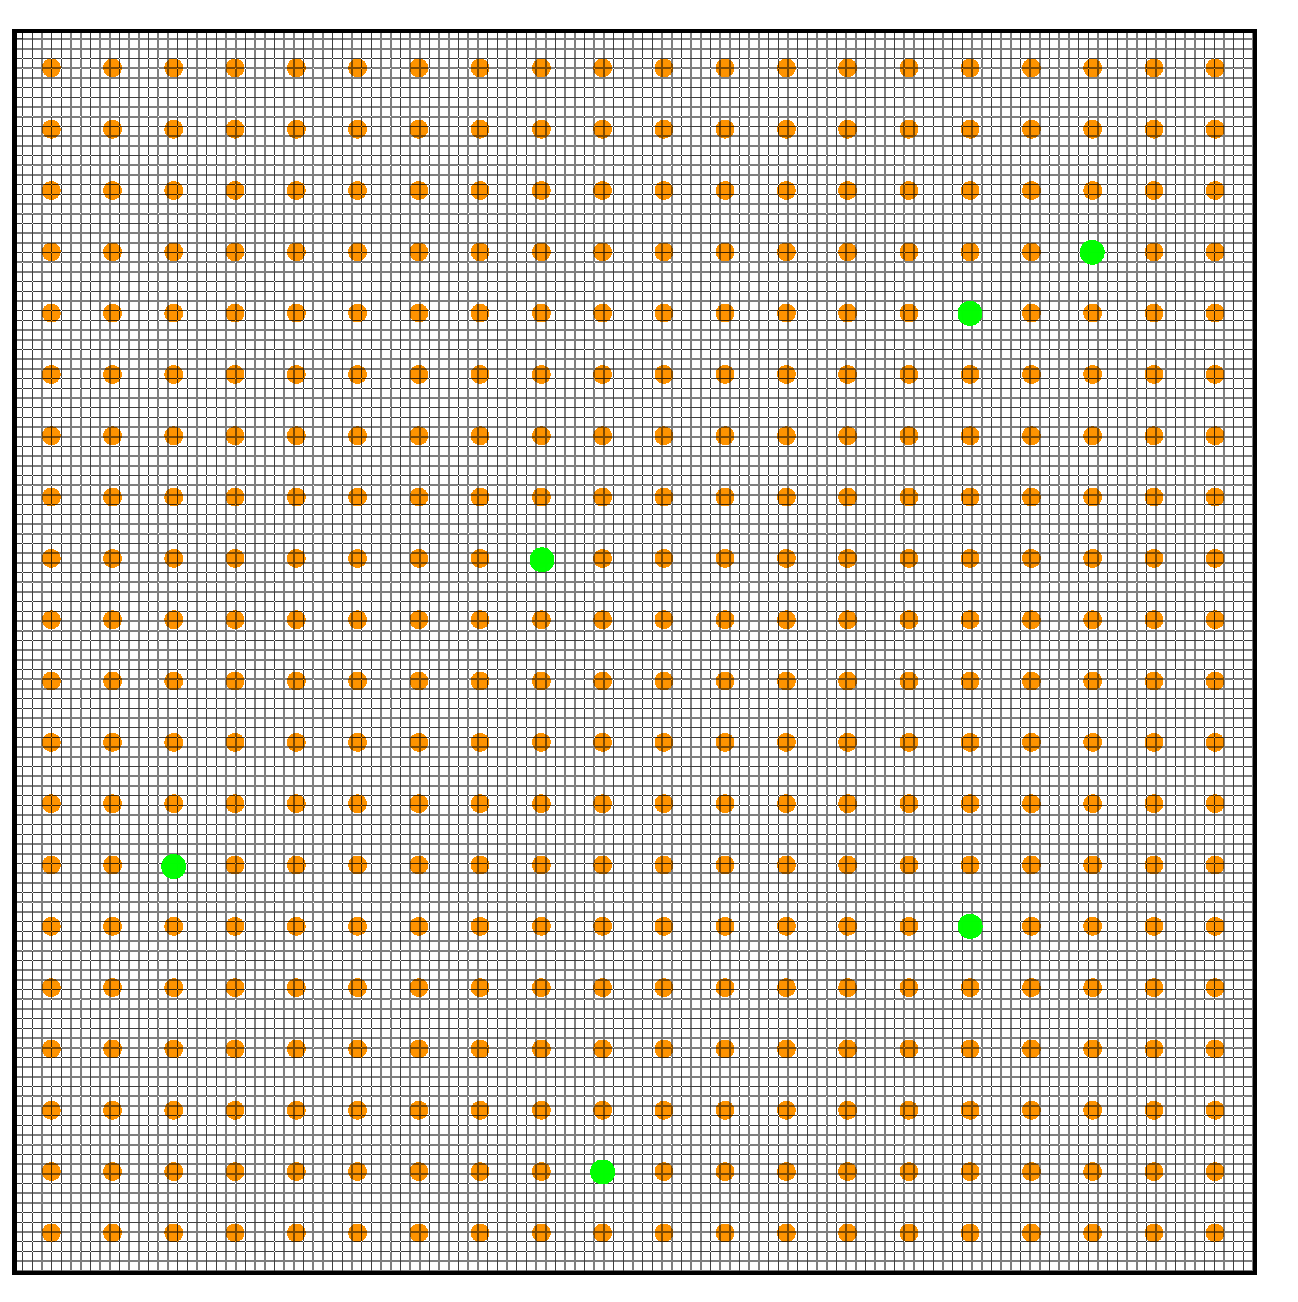
\includegraphics[width=\textwidth]{Ch5_QPIsim_demo.pdf}
	\caption{schematics for the simulation, in the actual calculation, we place defect at locations defined by lattice points, and compute $\delta\rho(\textbf{x},\omega)$ at each spatial grid point (128 by 128 here)}
	\label{fig:ch5_qpisim_demo}
\end{figure}

We first performed a single defect calculation, where we place the defect at the center of a square lattice with $51\times51$ sites, $\delta\rho$ was numerically computed at a $301\times301$ grid chosen to overlap with the square lattice, with defect energy $E_d$, hopping parameter $t$, onsite energy $E_0$. In total, 41 energy slices are computed in an energy range of $(-0.5, 0.5)V$.  

Typical \ac{LDOS} maps at different energy are shown in \ref{fig:ch5_single_scattering}, the figures are plotted on a gray scale image with the contrast indicating the level of \ac{LDOS} modulation. From the figures, we can make several observations:
\begin{itemize}
	\item The \ac{LDOS} modulation is featured by wave-like pattern similar to the Friedel oscillation we seen, and the pattern varies with energy.
	\item 2. The modulation is strongly correlated with the underlying lattice corrugation. 
	\item 3. Although the feature is decaying away from the defect location, the wave extend far into the space, indicating a relatively long life-time of this quasiparticle. And the life-time is especially long around the Fermi level, this aligns with our understanding about the Landau quasiparticle. 
	\item 4. The pattern persists further for patterns near the Fermi level. 
\end{itemize}




\begin{figure}
	\centering
	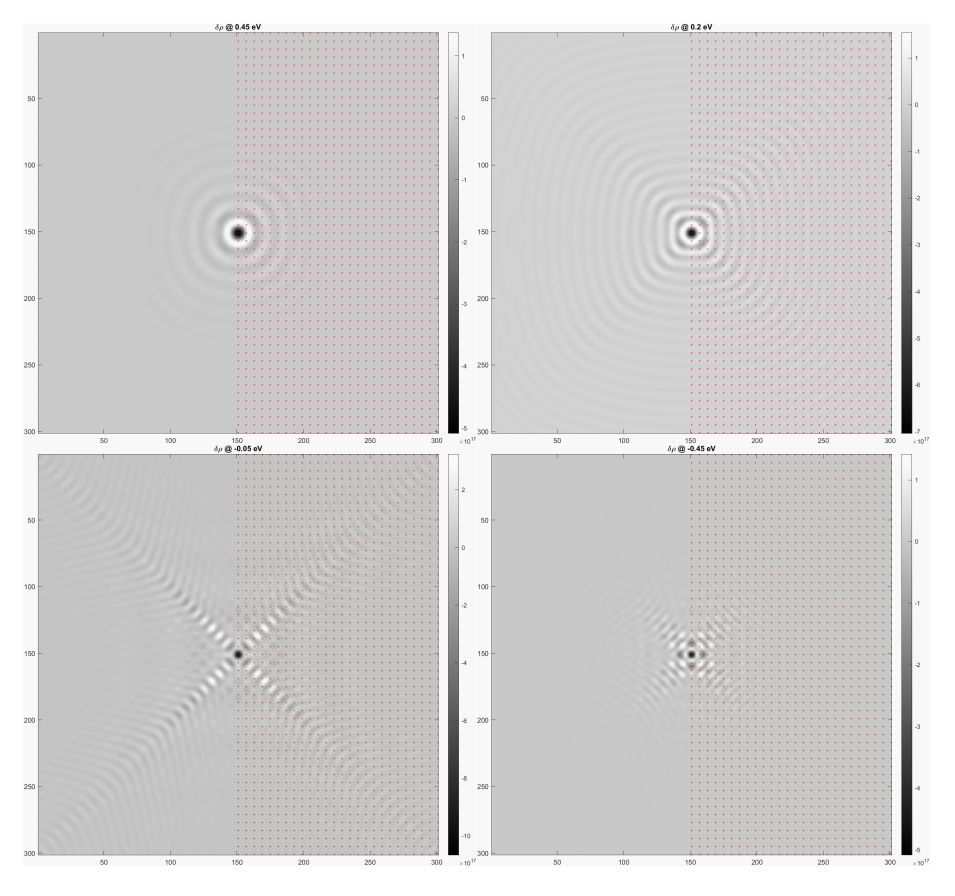
\includegraphics[width=\textwidth]{Ch5_singe_defect.png} % Replace with your image file
	\caption{$\delta\rho(\textbf{x},\omega)$ for single defect at the center of the 51 by 51 lattice grid with t = -0.2 and $\omega$ = 0.45, 0.20, -0.05 and -0.45 eV; the integrand size is defined by n = 300, $\epsilon = 1*10^{-3}$. }
	\label{fig:ch5_single_scattering}
\end{figure}

\begin{figure}
	\centering
	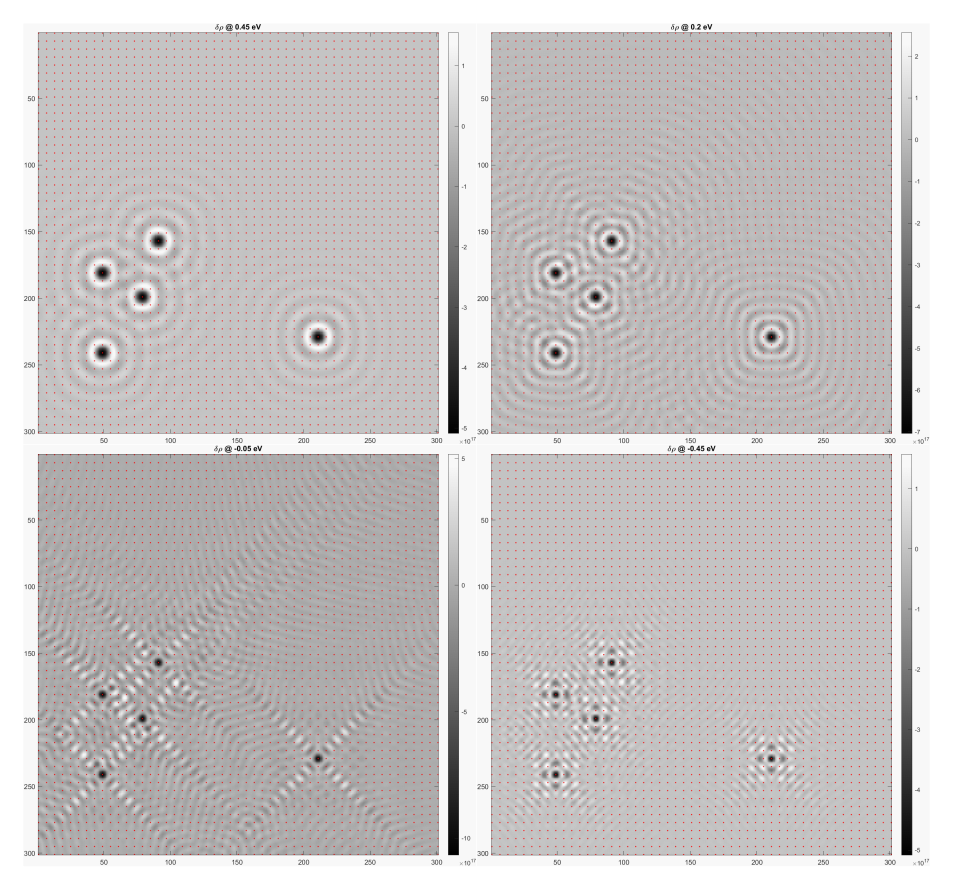
\includegraphics[width=\textwidth]{Ch5_multi_defect.png} 
	\caption{$\delta\rho(\textbf{x},\omega)$ for 5 randomly placed defect on the 51 by 51 lattice grid with t = -0.2 and $\omega$ = 0.45, 0.20, -0.05 and -0.45 eV; the integrand size is defined by n = 300, $\epsilon = 1*10^{-3}$. }
	\label{fig:ch5_multi_scattering}
\end{figure}

We also calculated multi-defect results, for this, the T-matrix is no longer a scalar but rather a real matrix capturing the correlation between defects. Numerical results are calculated with Equation \ref{multi_defect_eq}, and shown in Fig. \ref{fig:ch5_multi_scattering}, 5 defect locations are randomly selected on the lattice points, we can see that the interference pattern from different defect sources are more prominent on spots with clustered defects. 


\subsection{Interpretation of QPI}
Quasiparticle-impurity scatterings give arise to \ac{QPI}. Interpretations of \ac{QPI} can be quite involved in real materials, but all the factors to consider can be characterized into 2 aspects: 1. the detailed quasiparticle states, and 2. the characteristics of the impurity. We will illustrate these aspects with the system we established for the simulation above. 
 
As mentioned in the start of Ch5.2, quasiparticles carry the same quantum numbers ($\textbf{k}$,$\sigma$) as the bare particles; Therefore, in an electronic system, quasiparticle states are dictated by the system's band structure. For the 2D Tight-binding model with only nearest neighbor hopping that we considered, the energy dispersion $\epsilon_{\mathbf{k}}$ is a parabola in $k_x$ and $k_y$ as denoted in \ref{E_k} and plotted in \ref{fig:ch5_bs} a). In an elastic quasiparticle-impurity scattering process, given our impurity is non-magnetic, we have the incoming state $\Psi(\textbf{k}_i,\sigma)$ and outgoing state $\Psi(\textbf{k}_f,\sigma)$, where $E_{\textbf{k}_f} = E_{\textbf{k}_i}$. To enforce elastic scattering, we can take a constant energy slice at a given energy, this reveals all possible states at that energy; This slice is normally referred as a \ac{CEC} of that particular energy. While real life materials can possess more complicated selection rules, in a single band situation as we formulated here, any state on the \ac{CEC} can be an initial or a final state in the scattering process; Mathematically, to describe the scattering vector $\textbf{q} = \textbf{k}_f -\textbf{k}_i$, we can take a self-convolution of the \ac{CEC}, which we can easily calculate and plot; This self-convolution is often referred as the \ac{JDOS} at the corresponding energy. An example is given at an energy close to the Fermi level in b),c) of Fig \ref{fig:ch5_bs}. 
\begin{figure}
	\centering
	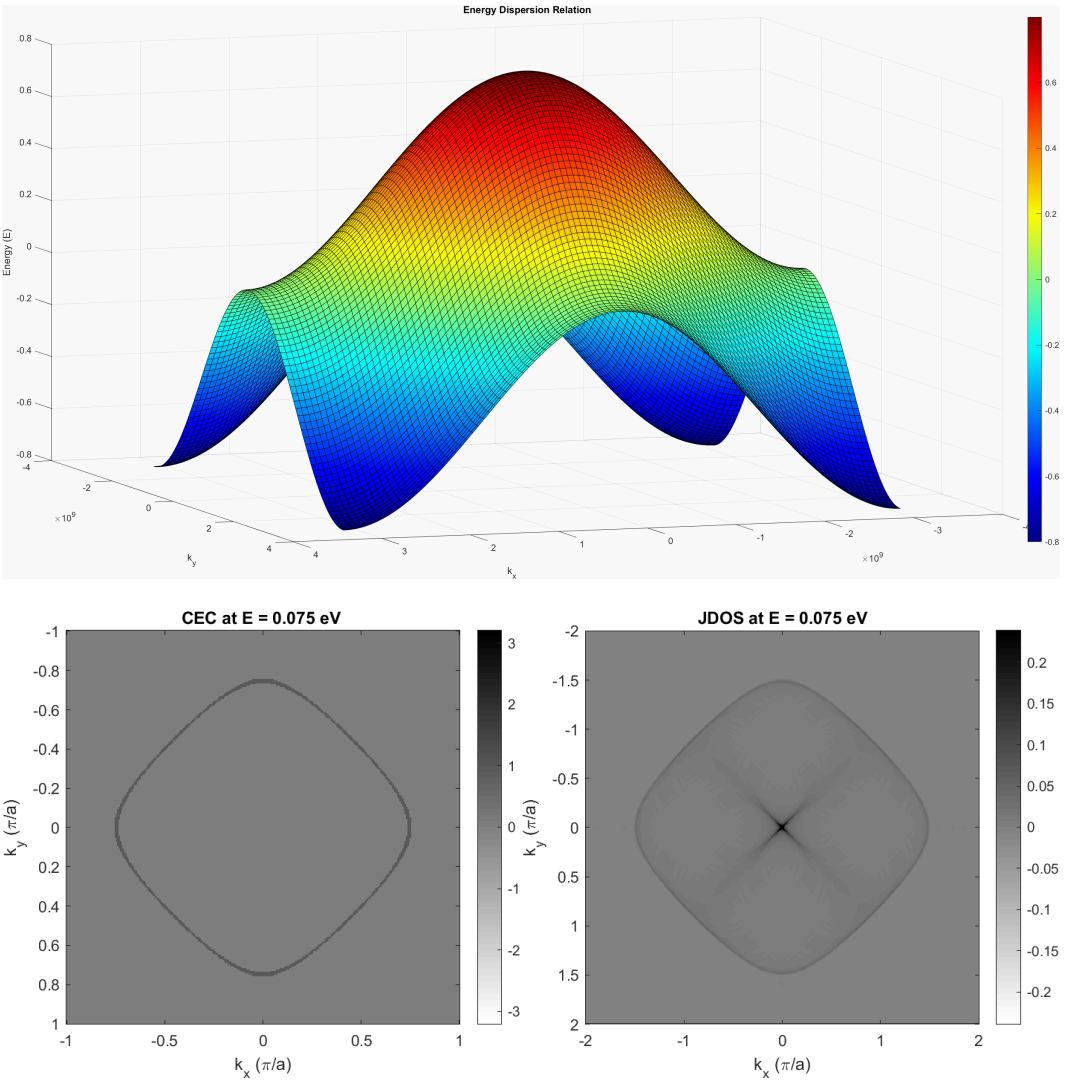
\includegraphics[width=\textwidth]{Ch5_BS_JDOS.png} 
	\caption{Band structure of 2D tight-binding square lattice with nearest neighbor hopping, a) 3D Energy dispersion in $\textbf{k}_x$ and $\textbf{k}_y$, b) Constant energy contour and c) Joint density of states at $E=0.075eV$}
	\label{fig:ch5_bs}
\end{figure}

The real space \ac{LDOS} modulation can now be interpreted, and we illustrate it with \ref{fig:ch5_ldos}. First, to focus us on the interference ripples, we suppress the features from the defect itself by apply a Gaussian masking at the defect location, a)-b). Then we apply the Fourier transform to get the \ac{QPI} map in reciprocal space as shown in c), the red dots in c) are the Bragg peaks of the system. As we know, the range in reciprocal space is inversely proportional to the real space resolution. Longer $\textbf{q}-space$ features correspond to high frequency features in the real space; In most materials, the wavelengths of ordering are confined by the lattice parameter, therefore, a common practice is truncate and keep the feature within the Bragg peaks, this gives us a closer look to the features as shown in d). 
\begin{figure}
	\centering
	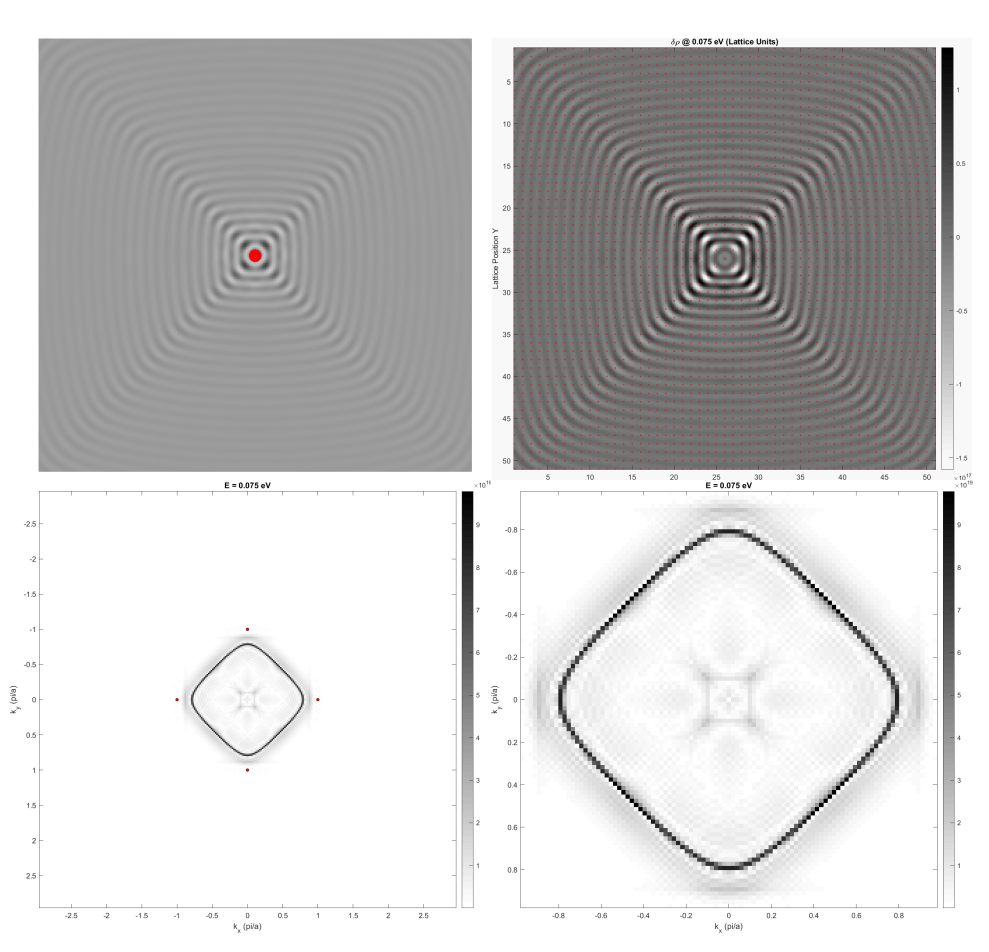
\includegraphics[width=\textwidth]{Ch5_LDOS_QPI.png} 
	\caption{Transfer QPI map from real-space to \textbf{q}-space, an example given at $E=0.075eV$, we first suppress the defect feature with a Gaussian mask at the red dot in a), this gives us b). We then apply 2D Fourier transformed to b) and get c), the red dots are indications of the Bragg peaks of the square lattice. d), \textbf{q}-space QPI map cropped within the Bragg peaks for better visibility of low-\textbf{q} features}
	\label{fig:ch5_ldos}
\end{figure}

We now make a direct comparison between the $\textbf{q}$-space \ac{QPI}, \ac{CEC} and \ac{JDOS}, as shown in Fig \ref{fig:ch5_compare}. We picked two $\textbf{q}$-vectors $\textbf{q}_1$ and $\textbf{q}_2$ in the $\textbf{q}$-space \ac{QPI}, by transferring them one to one into the \ac{CEC}, we can map two sets of initial and final momentum states. For each $\textbf{q}$-vector, we have $\textbf{q} = \textbf{k}_2 - \textbf{k}_1$. 
\begin{figure}
	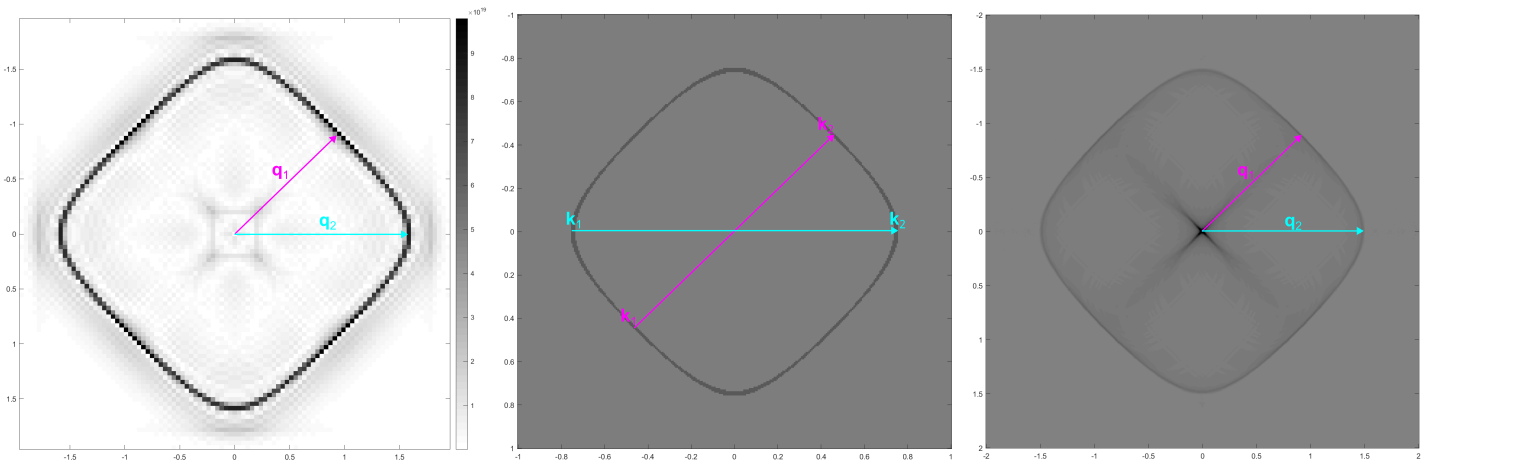
\includegraphics[width=1.1 \textwidth]{Ch5_QPI_JDOS.png} 
	\centering
	\caption{Interpretation of scattering vectors in \textbf{q}-space QPI map. Two \textbf{q}-vectors at horizontal and diagonal directions are drawn from the center to the high-intensity spots in a). b) is the \ac{CEC} in \textbf{k}-space at the same energy as a), states are binary in the \ac{CEC}, the darker gray indicates the presence of a state and lighter gray indicates the absence of a state. 2 arrowed lines of the corresponding colors indicates the scattering process from state in $\textbf{k}_1$ to state in $\textbf{k}_2$. c).\ac{JDOS} at the same energy, arrowed lines are in-scale with the lines in a) and b).}
	\label{fig:ch5_compare}
\end{figure}

There are two features in $\textbf{q}$-space \ac{QPI} that are worth mentioning: First, nested \ac{CEC} creates more concentrated intensity in $\textbf{q}$-space \ac{QPI}. Nesting is a term given to an energy iso-surface where there are surfaces with even spacing. In a two-dimensional system, we say a \ac{CEC} is nested when we have pairs of lines that have the same separations; Scattering between the states living on these lines gives the same $\textbf{q}$-vector and thus a concentrated intensity there. We can see this effect more clearly with a comparison as shown in Fig \ref{fig:ch5_compare}; Compare a) and c), we have a less faceted contour in c), and the resulting $\textbf{q}$-space \ac{QPI} has more spread out intensity. 

\begin{table}
	\centering
	\begin{tabular}{|c|c|c|c|}
		\hline
		Energy (eV) & Width ($\pi/a$) & Width Uncertainty ($\pi/a$) & R-squared \\
		\hline
		-0.5 & 0.0661 & 0.0044 & 0.9689 \\
		-0.4 & 0.0496 & 0.0040 & 0.9715 \\
		-0.3 & 0.0383 & 0.0034 & 0.9724 \\
		-0.2 & 0.0300 & 0.0028 & 0.9767 \\
		-0.1 & 0.0274 & 0.0032 & 0.9814 \\
		\hline
		0.075 & 0.0201 & 0.0014 & 0.9964 \\
		0.1 & 0.0328 & 0.0145 & 0.8706 \\
		0.125 & 0.0214 & 0.0013 & 0.9958 \\
		0.2 & 0.0286 & 0.0065 & 0.9350 \\
		0.3 & 0.0311 & 0.0048 & 0.9635 \\
		0.4 & 0.0392 & 0.0051 & 0.9544 \\
		0.5 & 0.0516 & 0.0062 & 0.9451 \\
		\hline
	\end{tabular}
	\caption{Horizontal profile fitting results showing the width and its uncertainty (in units of $\pi/a$) along with the R-squared values for both positive and negative bias energies.}
	\label{tab:qpi_fit_results_combined}
\end{table}

Secondly, the quasiparticle lifetime decreases as we move away from the Fermi surface. Given the momentum dependence of $\operatorname{Im}{\Sigma_{\textbf{k},\sigma}(\omega+i \eta)}$ is negligible, which is usually true, the spectral function is a simple Lorentzian in $\textbf{k}$-space of width $\operatorname{Im}{\Sigma}$ \cite{wolfleQuasiparticlesCondensedMatter2018}; Therefore, the \textbf{q}-space quasiparticle peak is also a Lorentzian with its width approximated at 2$\operatorname{Im}{\Sigma}$. Note that $\operatorname{Im}{\Sigma}$ is inversely proportional to the quasiparticle lifetime $\tau_{life}$, thus, we can probe $\tau_{life}$ by analyzing the broadening of the quasiparticle peaks in $\textbf{q}$-space \ac{QPI} at different energies. As shown in \ref{fig:ch5qplifetime}, we first take a horizontal line profile on the \textbf{q}-space \ac{QPI} that goes through the center, then fit a Lorentzian function on the quasiparticle peak region shown in the green dots in b), we can extract the peak width with its uncertainty. We then apply this process through different energy slices, the results are presented in Table \ref{tab:qpi_fit_results_combined} and plotted in c) of Fig. \ref{fig:ch5qplifetime}. All fittings possess a R-square value greater than 0.90 except for $E=0.1$, we thus marked the datapoint red in the plot. Quasiparticle peaks broadened as the energy deviated from the Fermi energy, however, within the energy range investigated, we still observe very sharp quasiparticle peaks, indicating long-lived and well-defined quasiparticles. 



\begin{figure}
	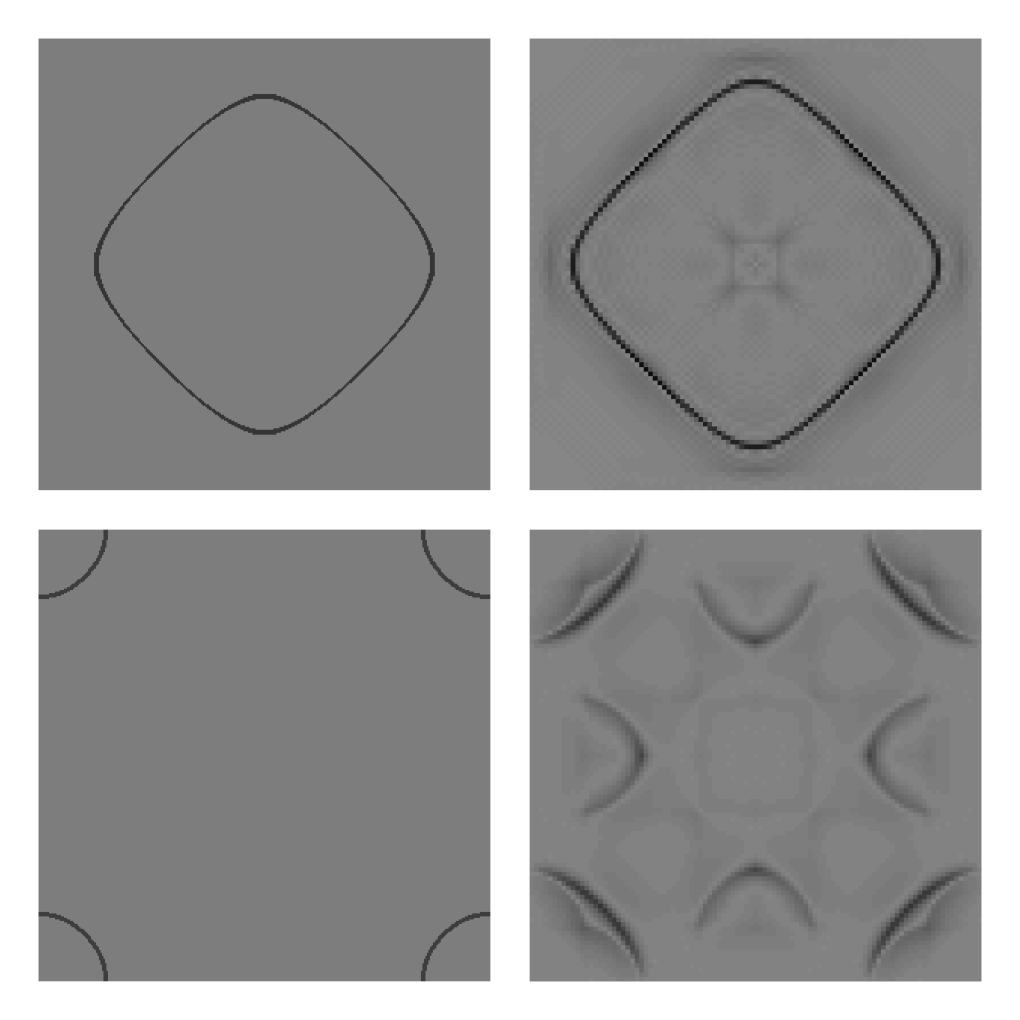
\includegraphics[width=\textwidth]{Ch5_nesting.png} 
	\centering
	\caption{Comparison of nesting effect on 2 energy slices of \textbf{q}-space QPI map, a more faceted \ac{CEC} like a) gives a more concentrated intensity in the QPI map b), compare to the unfaceted \ac{CEC} like c) gives a more spread out intensity in d).}
	\label{fig:ch5_nest}
\end{figure}


\begin{figure}
	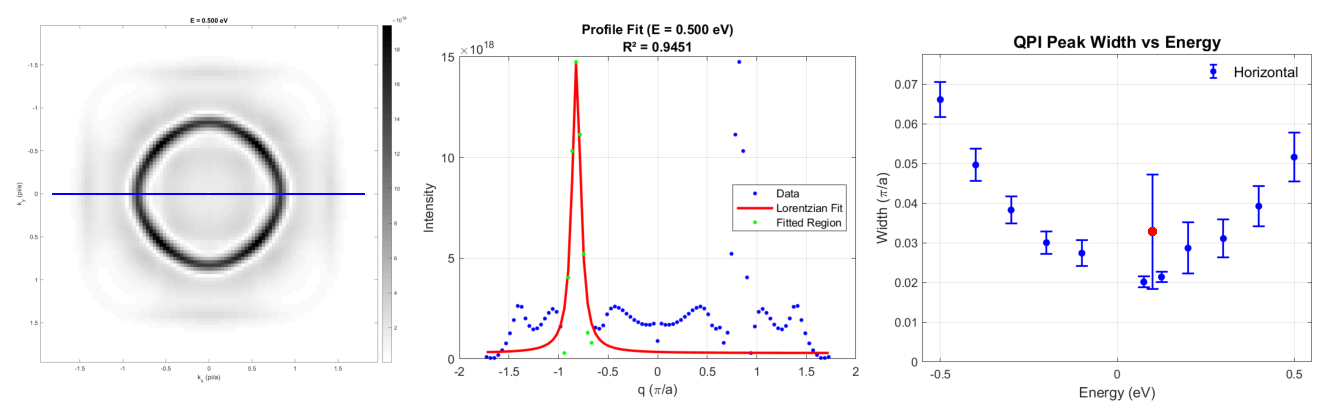
\includegraphics[width=\textwidth]{Ch5_qp_lifetime.pdf} 
	\centering
	\caption{Fitting quasiparticle peaks with Lorentzian and extract the width at different energy levels. a)-b) An illustration of the process, we first extract the horizontal profile of the QPI map, then we identify two peaks in the profile, by symmetry argument, we fit one peak with Lorentzian function. c) QPI peak width across different energies, we see that as energy moves away from the Fermi level, the peaks broaden and $\tau_{life}$ decreases.}
	\label{fig:ch5qplifetime}
\end{figure}

Finally, it is important to note that different defect configurations will result in different \ac{QPI} patterns. This is due to gauge-field phase sensitivity in \ac{QPI}. As a scattering process, the quasiparticle state not only exchanged momentum with the impurity, it also picks up an additional phase $\delta$ during the process; Thus, certain QPI peaks can be suppressed if the phase shift due to scattering mismatches the phase difference between the two states. Moreover, this relative phase depends on the nature of the defects, similar to the refractive phase picked up by photon changes for different interface material, different defects will suppress \ac{QPI} intensities in different ways, give arise to different \ac{QPI} patterns. 
%todo: maybe we can talk about the phase effect from impurity configuration. 


%Estimating the multidefect result with convolution approach inherently makes assumption into the independent nature of scattering, which is only true for weak scattering and sparse impurity distributions. 


\section{Experimental QPI measurement}
Realspace \ac{QPI} signals are obtained by taking the grid map experiment on a region that presents \ac{QPI} patterns. In this section we will briefly explore \ac{QPI} measurement in the \ac{STM} experiment, more specifically, we will introduce the factors that dictate \ac{QPI} quality, discuss how to choose proper parameters that result in a good \ac{QPI} measurement, and finally we will present a specific challenge called the phase noise, which motivates our work in the next chapter.


\subsection{QPI measurement and quality}
As mentioned in Ch.2, taking a grid map is very involved. A successful grid map requires both an ideal instrumental setup and a set of proper measurement parameters based on the understanding of the targeting material. 

The key objective of an ideal instrumental setup is to create a stable environment and lower the system noise; as we discussed in Ch.2, this involves minimizing the noise from mechanical vibration, temperature fluctuation, and electronic instability of the system and maintaining a stable tip-surface tunneling junction. 

A grid map is defined by a $N\times N$ (assuming square) grid on a targeted area of $L \times L$ $nm^2$, this provides a spatial resolution $\Delta L = \frac{L}{N}$; In reciprocal space, this set up gives a range $Q = \frac{2 \pi}{\Delta L}$ with resolution $\Delta Q = \frac{2\pi}{L}$, the energy range and resolution is defined by the setting of the single-point spectroscopy performed on every grid point. 

A set of proper parameters for \ac{QPI} measurement aims to extract the most amount of information with the highest level of resolution given the constraints of the system. The most important constraint is the limiting cryogenic holding time. This puts a ceiling on the grid map run time, while different systems vary; typically, the cryogenic holding time is a fraction of a week. Within the boundary of the run time, we usually aim for a grid with a fine reciprocal resolution $\Delta Q$ and a reasonable reciprocal range $Q$, corresponding to a large field of view $L$ and a reasonable $\Delta L$. It is intuitive to have a proper size of reciprocal range $Q$ that is not infinitely large, as most of the q-space features reside within the Bragg peaks, exemplified by Fig. \ref{fig:ch5_ldos} c). But we also do not want the field of view $L$ to be too large, this is because in real experiments with finite noise level, the featured \ac{QPI} pattern has a finite lifetime and its intensity will dive under the noise at some cutoff distance $r_{cutoff}$ from the defect center; Thus, a field of view larger than the cutoff distance will instead decrease the signal to noise ratio. We illustrate cutoff distances in systems with different noise levels in Fig. \ref{fig:ch5_cutoff}. The noise level is set to be noiseless, SNR = 10, and SNR = 1.2, respectively; given the noise level shown in the green dotted line, we identify the furthest signal peak higher than the noise level and place a blue vertical line there. These vertical lines indicate the cutoff distances; and we can see with increasing noise level, $r_{cutoff}$ drops, and thus the optimal field of view should also drop.  

\begin{figure}
	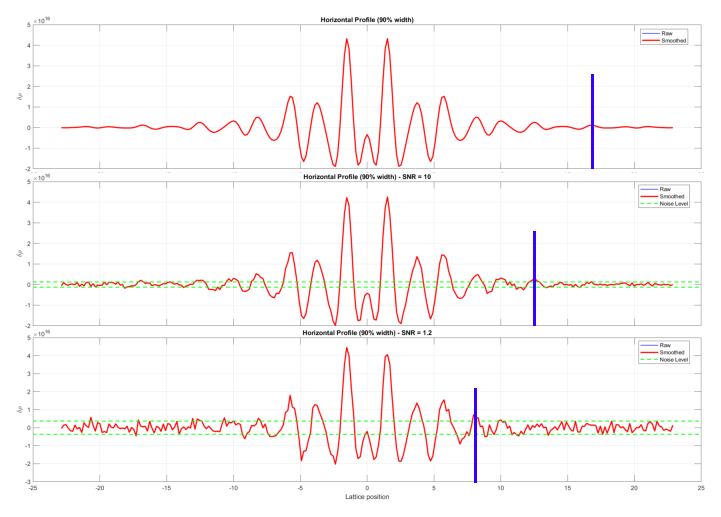
\includegraphics[width=\textwidth]{Ch5_fieldofview.pdf} 
	\centering
	\caption{Cutoff distances of QPI patterns with different signal-to-noise ratios. Three Horizontal Line profiles on $\delta\rho(\textbf{x}, E=0.45eV)$ with the noise of various levels. a) has no noise applied; b), c) have Gaussian noises applied with SNR = 10 and 1.2, respectively. Here the signal strength is defined as the variance of the noiseless $\delta\rho(\textbf{x}, E=0.45eV)$, see a) of Fig. \ref{fig:ch5_single_scattering}.}
	\label{fig:ch5_cutoff}
\end{figure}


\subsection{multi-defect QPI pattern and phase noise}
\ac{QPI} patterns present themselves around defects. While an ideal \ac{QPI} measurement is performed on isolated defects in a large field of view, it is normally difficult to find such a case. In real experiments, grid maps are usually taken on areas with multiple defects; this causes interference between the \ac{QPI} patterns originating from different defects, as hinted by Ch.5.2.4 when discussing Fig. \ref{fig:ch5_multi_scattering}.

This is problematic when we try to interpret the \textbf{q}-space \ac{QPI} map. As illustrated in Fig. \ref{fig:ch5_phasenoise}, when we have multiple defects scattered in the field of view, we start to see some noise patterns associated with the spatial distribution of the defects, as we can see by comparing c) and e), we see that with nothing but the relative locations of the defects changed, the corresponding \textbf{q}-space \ac{QPI} maps possess different noise patterns. This effect is called phase noise; it hinders our ability to analyze the underlying quasiparticle scattering process. 

\begin{figure}
	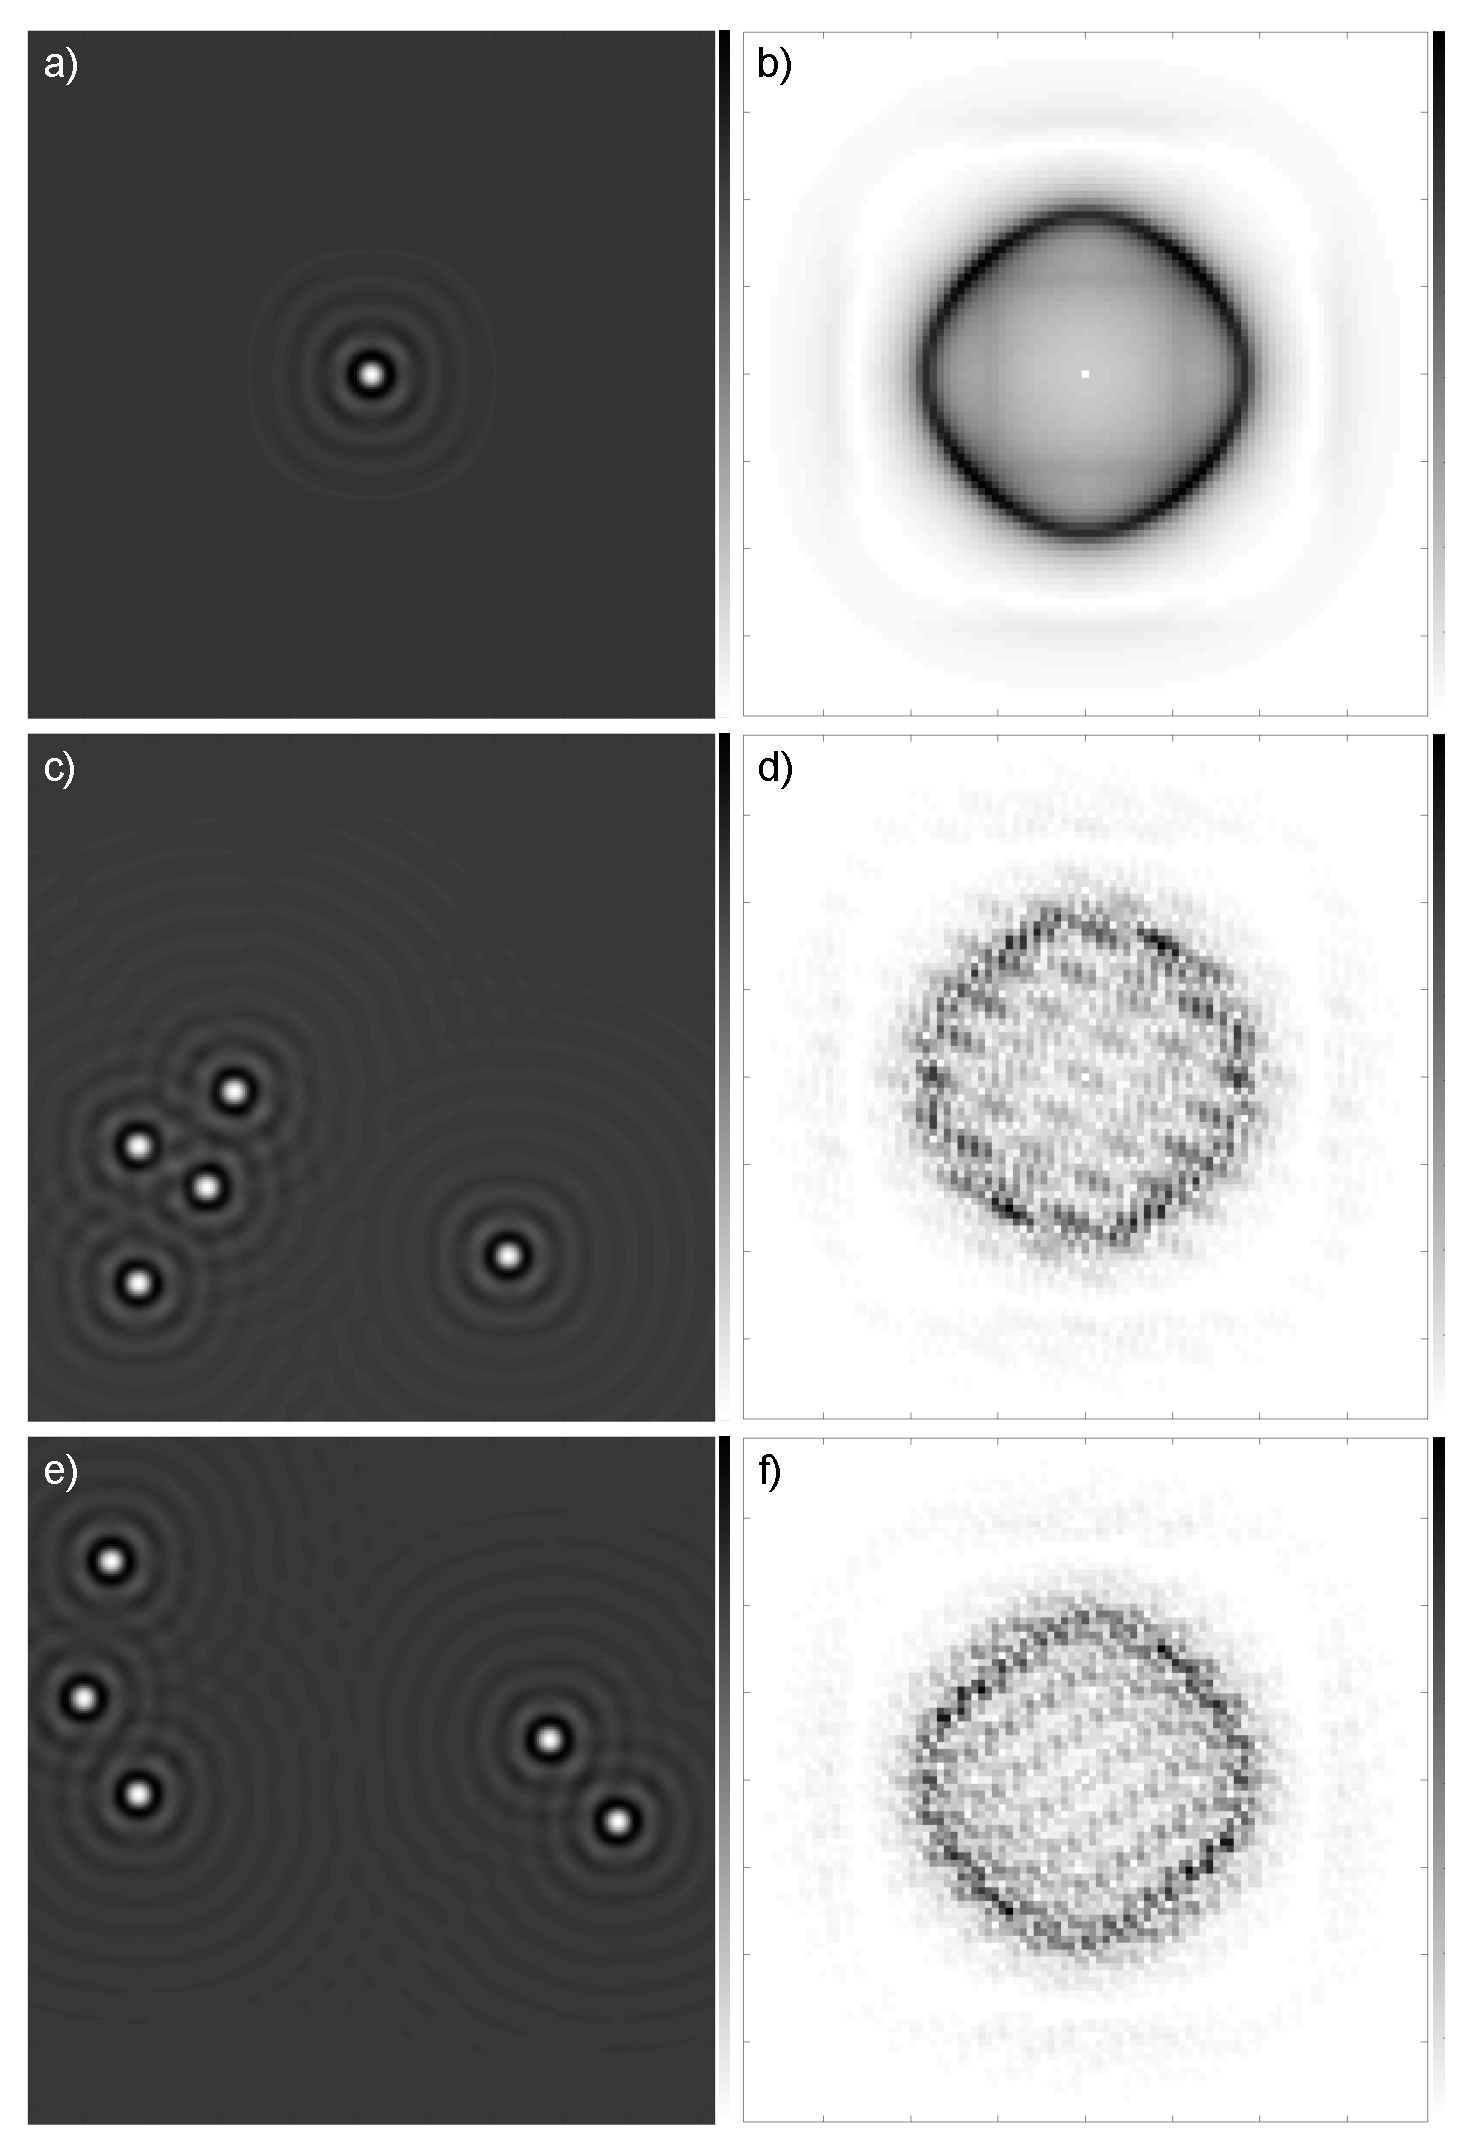
\includegraphics[width=0.85 \textwidth]{Ch5_phasenoise.pdf} 
	\centering
	\caption{Phase noise illustration. a),b): single defect scattering pattern and corresponding \textbf{q}-space QPI map. c)-f): multi-defect scattering with the same number of defects with different distributions, the corresponding QPI map presents phase noise with different patterns that associate with the defect distribution}
	\label{fig:ch5_phasenoise}
\end{figure}

Beyond the phenomenological illustration, we can further understand the source of phase noise with a mathematical analysis on multi-defect $\delta\rho(\textbf{x},\omega)$. We first discuss the form of the multi-defect T-matrix T, which is a $N_d \times N_d$ square matrix with entry T$_{\alpha \beta}$ representing the cross scattering term between defect m and n. We then separate the diagonal and off-diagonal terms and express T as\cite{leonard1972}:
\begin{align}
	\ T_{\alpha\beta} &= t_{\alpha} \delta_{\alpha\beta} + t_{\alpha} G_{0\alpha\beta} (1 - \delta_{\alpha\beta}) t_{\beta} + \sum_{\alpha' \neq \alpha, \beta} t_{\alpha} G_{0\alpha\alpha'} t_{\alpha'} G_{0\alpha'\beta} t_{\beta} + \cdots \label{eq_tmul}\\
	\label{eq.536}
	&= t_{\alpha} \delta_{\alpha\beta} + t_{\alpha} \sum_{\alpha'} \check{G}_{\alpha\alpha'} \ T_{\alpha'\beta},
\end{align}
\noindent where $t_{\alpha}$ is the T-matrix of a single impurity at site $\alpha$ and expressed on a matrix form in a localized basis set (i.e., expressed as the matrix with the same dimension as the multi-defect case but with only the $\alpha$'s diagonal entry none empty). And matrix $\check{G}_{\alpha\alpha'} = G_{0\alpha\alpha'}(1-\delta_{\alpha\alpha'})$, it contains the off-diagonal part of the Green's function. It has been shown by Fang et al. \cite{fangTheoryQuasiparticleInterference2013} that, in the Born approximation to the scattering amplitude, the first term dominates over the second term, and the latter can be omitted. We can, therefore, approximate multi-defect scattering with multiple single-defect scattering events. 

This approximation was then extended to the strong scattering case by Philipp et al. \cite{russmannInitioTheoryFourierTransformed2021}, under the assumption that the impurity concentration is low and the largest part of the surface is covered by pristine atoms and far from the impurities. They then utilized Equation \ref{eq.536} and further expressed the Green's function difference:

\[
\Delta G(\mathbf{r}, \mathbf{r}, E) = \int d^3 \mathbf{r}' \int d^3 \mathbf{r}'' \, G_0(\mathbf{r}, \mathbf{r}'; E) \, T(\mathbf{r}', \mathbf{r}''; E) \, G_0(\mathbf{r}'', \mathbf{r}; E)
\]

\begin{align}
	\label{eq.537}
	\Delta G_{\alpha \alpha} &= \Delta G^{(1)}_{\alpha \alpha} + \Delta G^{(2)}_{\alpha \alpha} \\
	\label{eq.538}
	&= \sum_{\alpha'} G_{0\alpha \alpha'} t G_{0\alpha' \alpha} + \sum_{\alpha'} G_{0\alpha \alpha'} t\sum_{\beta \beta'} \check{G}_{\alpha' \beta} \, T_{\beta \beta'} G_{0\beta' \alpha}.
\end{align}

\noindent By applying the stationary phase approximation \cite{lounisTheoryRealSpace2011} to $G_{0\beta'\alpha}$, and utilize the transnational symmetry of Bare lattice Green's function $G_0$, they showed:
\[
\Delta G^{(2)}_{\alpha\alpha}=\sum_{\alpha'}G_{0\alpha\alpha'}t\sum_{\beta\beta'}\check{G}_{\alpha'\beta}T_{\beta\beta'}K_{\beta'\alpha}e^{ik_{\beta'\alpha}\cdot R_{\beta'\alpha}},
\]
\noindent where the contribution of the last phase, $e^{ik_{\beta'\alpha}\cdot R_{\beta'\alpha}}$ can not be lifted, and is thus the source of the phase noise we observed in Fig. \ref{fig:ch5_phasenoise}. 

It is further noted that the contribution of the phase can be piratically canceled if we sum over all configurations of randomly distributed defects, which correspond to an infinitely large scanning surface, which can never be achieved. However, a decreased influence of this phase noise can be seen if we increase the density of the defects, as illustrated in Fig \ref{fig:ch5_changephasenoise}. This is because the patterns created by the phase noise become more fine-grained and can eventually be seen as featureless, similar to the random distribution of noise.  
%todo: verify whether this is true with more literature reviews. 

\begin{figure}
	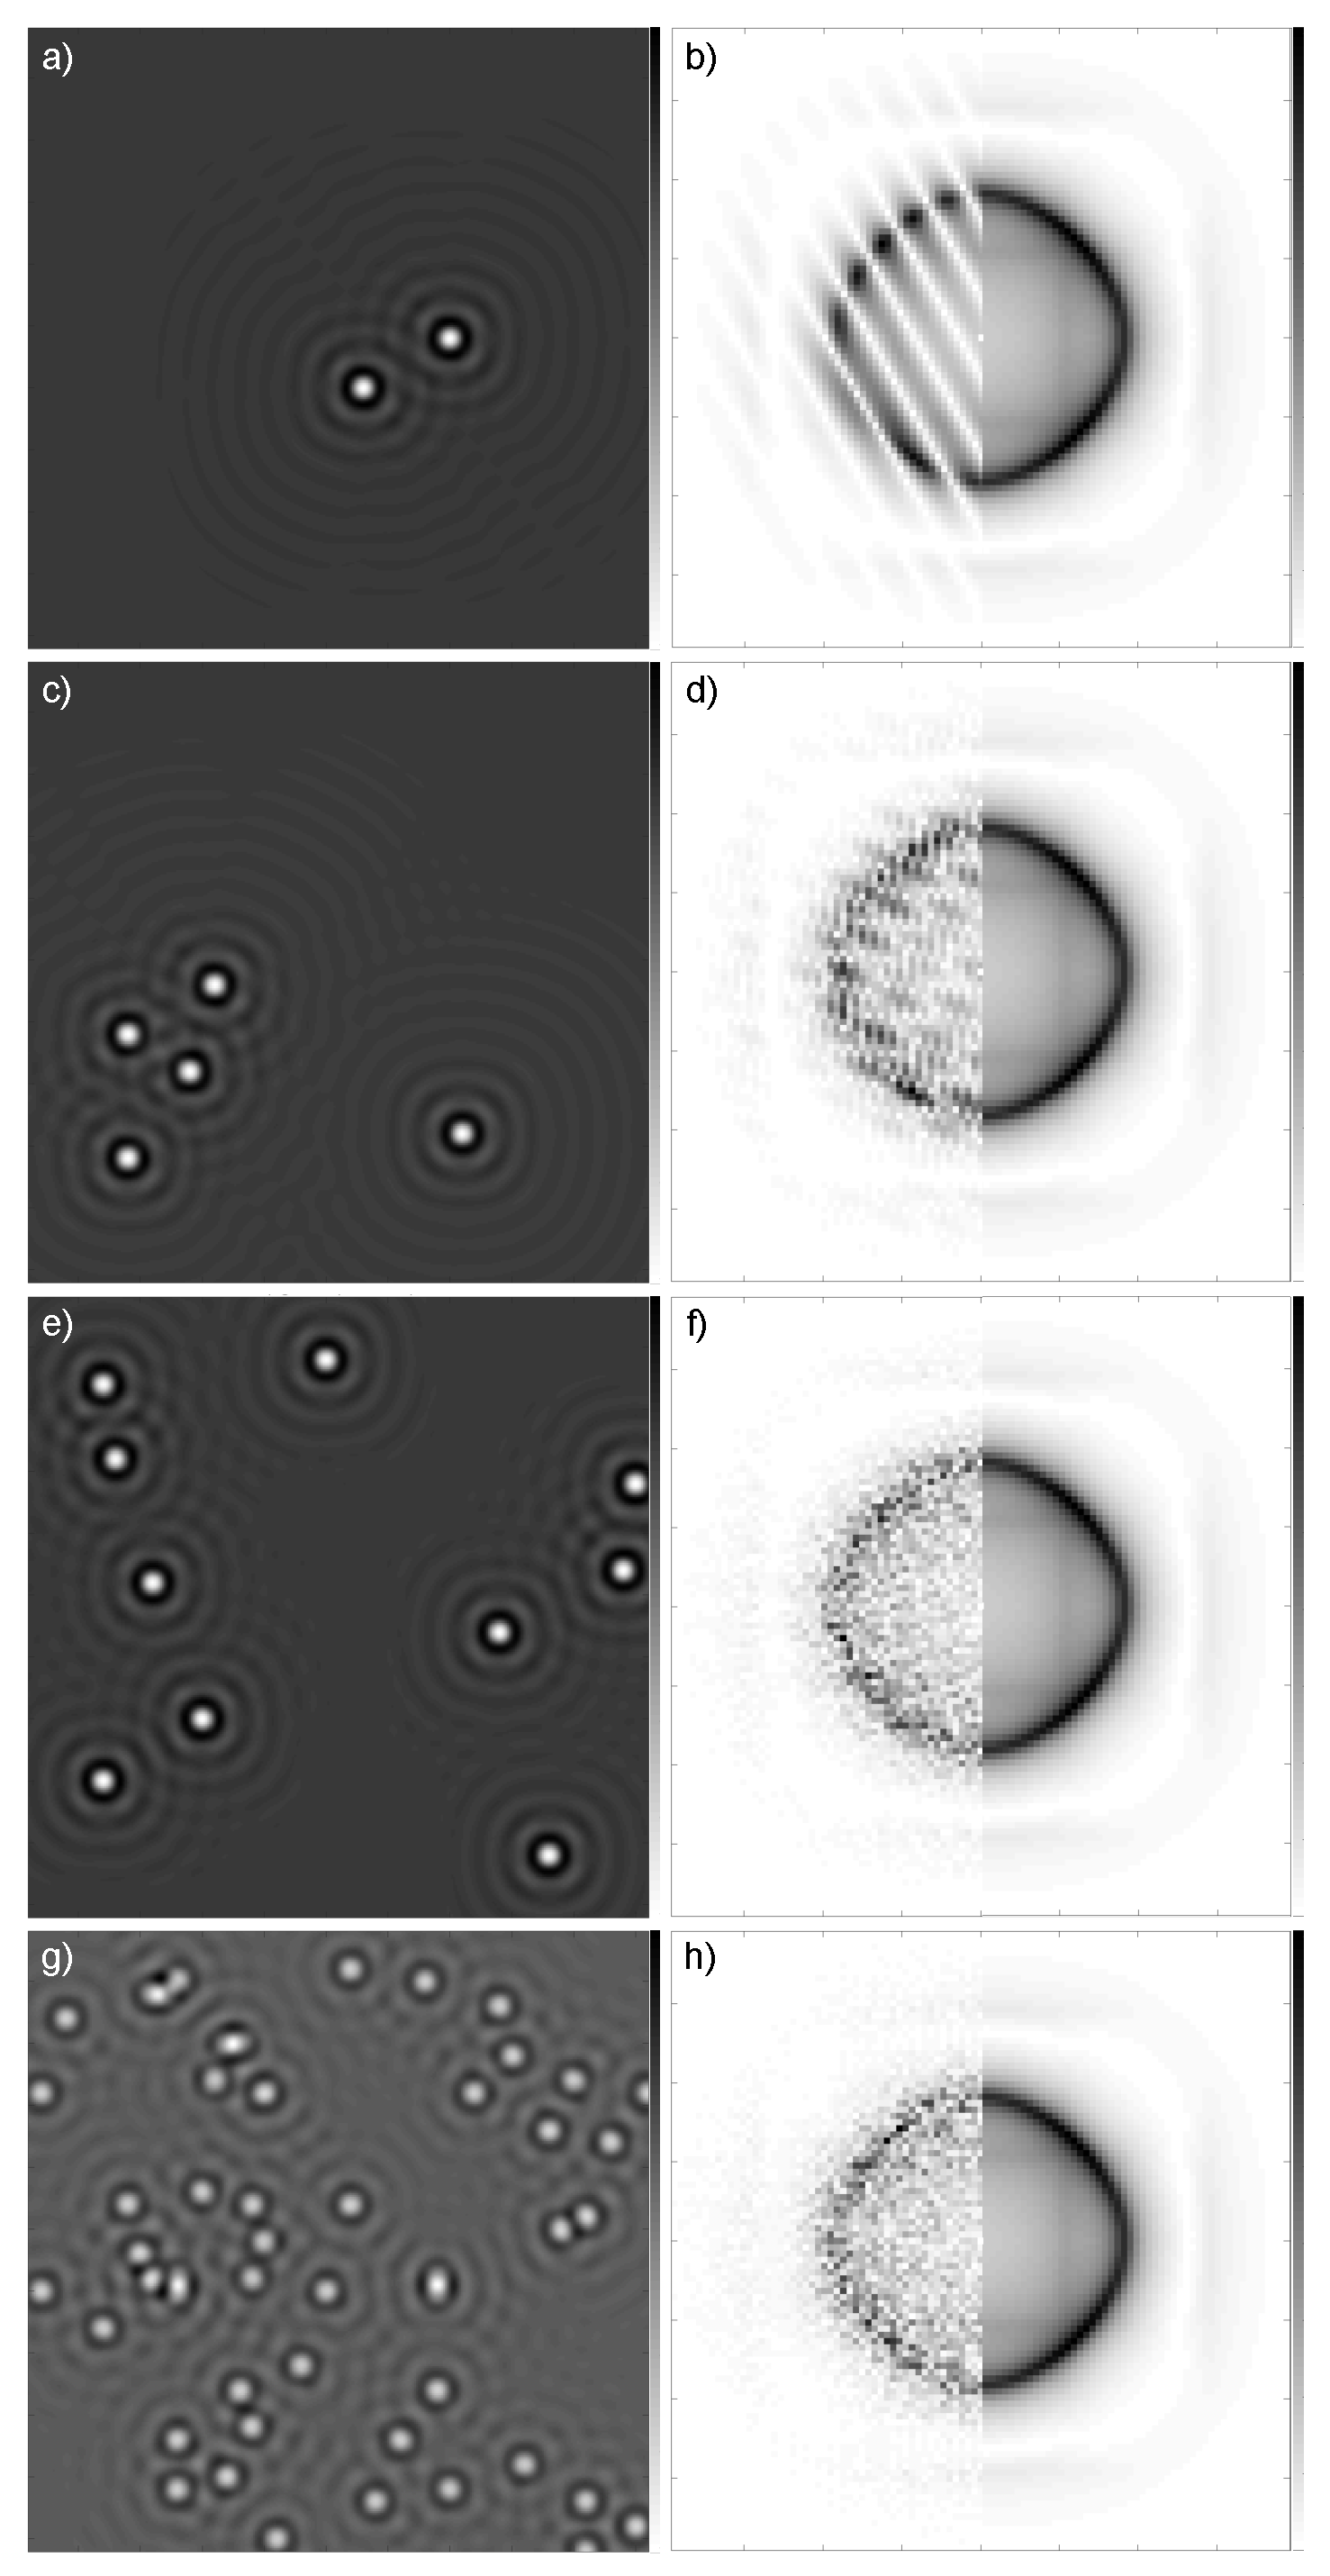
\includegraphics[width=0.7 \textwidth]{Ch5_changephasenoise.pdf} 
	\centering
	\caption{The effect of the phase noise is most prominent in the sparse defects regime. a)-h): $\delta\rho(\textbf{r},\omega)$ and \textbf{q}-space QPI plotted in pair with increasing defect concentration, showing the phase noise becomes more featureless. Single-defect QPI map is presented for reference on the right half of the \textbf{q}-space QPI.}
	\label{fig:ch5_changephasenoise}
\end{figure}


\section{Existing Algorithm}
\subsection{Shortcomings of existing algorithm}
\begin{itemize}
	\item 1. Their simulation data used truncated QPI pattern, not true to the real STM case. 
	\item 2. Too ideal to be useful in most cases ho
\end{itemize}
\subsection{Out mitigation}
To avoid truncated QPI pattern, during simulation. There are a few things to keep in mind: 
\begin{itemize}
	\item 1. Forming observation by 2d convolution of activation and single defect QPI pattern is much time/computationally efficient to work with, than directly simulate multi defect QPI pattern. 
	\item 2. So we will use single defect QPI pattern. 
	\item 3. To simulate single defect QPI pattern, we will need to define, apart from physical constants: a. n$_l$: number of lattice points along one dimension. b. n$_p$: number of pixels of this simulation in one dimension. From a, b we can then compute the grid resolution pixel/nm that this simulation correspond to in physical system, for instance given a lattice parameter a, then for our kernel, we have grid resolution = a*n$_l$/n$_p$ nm/pixel.
	\item 4. Note that a physical activation is nothing but a r*r square lattice span some real space area of $(r*a)^2$with N$_d$ number of defect located on some of the lattice points. However, in simulation activation, we have a matrix of n*n that on each point there is a certain probability it is a defect site, this means, here n has the same physical meaning as r.
	\item 5. $Y=conv2d(X,A)$ but this convolution assumes that we have the kernel's resolution same as the activation. To make that assumption hold, we need the activation's resolution = lattice constant/pixel = a nm/pixel, then we need to have n$_l$ = n$_p$. However, this case we lost the flexibility of changing or activation resolution. Another case is to let the activation holds the same resolution to the kernel, which is conventionally arbitrary, and this is also problematic as this case we are allowing defects sitting not on their lattice site, which is only true for defects like interstitial.
	\item The ideal case would be, the  activation resolution/kernel resolution is an integer, meaning n$_l$/n$_p$ =q, q is an integer. Then we should have a fake activation whose side = n*q, where as defects are only allowed to sit in the real activation whose side is n.
\end{itemize}
Then how do we determine the window size? it really 
\section{SBD-STM Performance Analysis}
\subsection{Analysis for Different Regimes for Scatter Density}
\subsection{Analysis for Dataset with Different Noise Structure}
\subsection{Analysis for Scattering with Long Coherent Length (Ag Dataset)}
\section{Multi-Type-Scatters (MT) SBD-STM}
	

\chapter{QPI on PtSn\textsubscript{4}}
\section{PtSn\textsubscript{4} Defect Scattering and QPI Data}
\footnote{Present Grid and QPI as Data, Orientation Determination and Preliminary Analysis}
\section{post MT-SBD-STM QPI analysis}
\subsection{Comparison with DFT Calculation}
\footnote{Follow-up with Nic on the Exact Model}

\chapter{MT-SBD-STM on other systems}
\section{Ag}
\section{ZrSiTe}